\documentclass[british]{scrreprt}

\usepackage{scrhack}
\usepackage{amsmath}
\usepackage{amssymb}
\usepackage{pifont}
\usepackage{fontspec}
\usepackage{unicode-math}
\usepackage[verbose = silent]{microtype}
\usepackage[urldate = iso, sortcites = true]{biblatex}
\usepackage[useregional]{datetime2}
\usepackage{csquotes}
\usepackage{epigraph}
\usepackage{graphicx}
\usepackage{pdfpages}
\usepackage{minted}
\usepackage{booktabs}
\usepackage{longtable}
\usepackage{siunitx}
\usepackage{threeparttable}
\usepackage{tabu}
\usepackage[hidelinks]{hyperref}
\usepackage{enumitem}
\usepackage{calc}
\usepackage{physics}
\usepackage[xindy, toc, numberedsection]{glossaries}
\usepackage{algorithm2e}
\usepackage{tikz}
\usepackage{pgfplots}
\usepackage{xcolor}
\usepackage[standard]{ntheorem}
\usepackage[nameinlink]{cleveref}
\usepackage{pdflscape}
\DeclareDocumentCommand{\todo}{m}{}
%\usepackage{luatodonotes}
\usetikzlibrary{external}
\tikzexternalize[
	prefix = tikz/,
	optimize command away = \includepdf,
	optimize command away = \todo
]

\KOMAoptions{
	abstract = true,
	chapterprefix = true,
}
\setkomafont{disposition}{\normalcolor\bfseries}
\renewcommand*{\chapterformat}{%
\mbox{\chapappifchapterprefix{\nobreakspace}\thechapter\IfUsePrefixLine{}{\enskip}}
}
\renewcommand{\chapterlineswithprefixformat}[3]{%
	\centering
	{\normalfont\textsc{#2}}\hrule\par\bigskip#3\par\bigskip\hrule%
}

% https://tex.stackexchange.com/a/313337/105667
\newlist{todolist}{itemize}{2}
\setlist[todolist]{label=$\square$}
\newcommand{\done}{\rlap{$\square$}{\raisebox{2pt}{\large\hspace{1pt}\ding{51}}}%
\hspace{-2.5pt}}
\newcommand{\wontfix}{\rlap{$\square$}{\large\hspace{1pt}\ding{55}}}

\setmainfont{TeX Gyre Pagella}
\setsansfont{Open Sans}
\setmonofont{Fira Code}
\setmathfont{TeX Gyre Pagella Math}

\renewcommand{\mkbegdispquote}[2]{\itshape}
\renewcommand{\mkenddispquote}[2]{#1\\\normalfont#2}
\renewcommand{\mkcitation}[1]{\textemdash~#1}

% https://tex.stackexchange.com/a/537722/105667
\newrobustcmd*{\citefullauthor}{\AtNextCite{\DeclareNameAlias{labelname}{given-family}}\citeauthor}

\setminted{
	autogobble = true,
	breaklines = true,
	tabsize = 2,
}

\sisetup{
	table-text-alignment = left,
	table-number-alignment = right,
}

\renewcommand\laplacian{\increment}
\newcommand\R{\mathbb{R}}

\makeglossaries
%\setacronymstyle{long-sc-short}
\newacronym{hpc}{HPC}{high-performance computing}
\newacronym[description = {Swiss National Supercomputing Centre}]{cscs}{CSCS}{Centro Svizzero di Calcolo Scientifico}
\newacronym{ssl}{SSL}{Scientific Software \& Libraries}
\newacronym[description = {Swiss Federal Institute of Technology}]{eth}{ETH}{Eidgenössiche Technische Hochschule}
\newacronym{ansi}{ANSI}{American National Standards Institute}
\newacronym{iso}{ISO}{International Organization for Standardization}

\definecolor{ETH1}{cmyk/RGB/HTML}{1.00, 0.70, 0.00, 0.30 /  31,  64, 122 / 1F407A} % dark blue
\definecolor{ETH2}{cmyk/RGB/HTML}{0.75, 0.40, 1.00, 0.40 /  72,  90,  44 / 485A2C} % dark green
\definecolor{ETH3}{cmyk/RGB/HTML}{1.00, 0.50, 0.00, 0.00 /  18, 105, 176 / 1269B0} % blue
\definecolor{ETH4}{cmyk/RGB/HTML}{0.30, 0.00, 1.00, 0.55 / 114, 121,  28 / 72791C} % green
\definecolor{ETH5}{cmyk/RGB/HTML}{0.20, 1.00, 0.00, 0.20 / 145,   5, 106 / 91056A} % magenta
\definecolor{ETH6}{cmyk/RGB/HTML}{0.00, 0.00, 0.00, 0.70 / 111, 111, 111 / 6F6F6F} % gray
\definecolor{ETH7}{cmyk/RGB/HTML}{0.00, 0.90, 0.80, 0.20 / 168,  50,  45 / A8322D} % red
\definecolor{ETH8}{cmyk/RGB/HTML}{1.00, 0.25, 0.30, 0.10 /   0, 122, 150 / 007A96} % cyan
\definecolor{ETH9}{cmyk/RGB/HTML}{0.00, 0.55, 1.00, 0.40 / 149,  96,  19 / 956013} % brown

\colorlet{ETHDarkBlue}{ETH1}
\colorlet{ETHDarkGreen}{ETH2}
\colorlet{ETHBlue}{ETH3}
\colorlet{ETHGreen}{ETH4}
\colorlet{ETHMagenta}{ETH5}
\colorlet{ETHGray}{ETH6}
\colorlet{ETHRed}{ETH7}
\colorlet{ETHCyan}{ETH8}
\colorlet{ETHBrown}{ETH9}

\definecolor{ETH180}{cmyk/RGB/HTML}{0.80, 0.52, 0.00, 0.24 /  56,  92, 155 / 385C9B}
\definecolor{ETH160}{cmyk/RGB/HTML}{0.60, 0.39, 0.00, 0.18 / 116, 141, 185 / 748DB9}
\definecolor{ETH140}{cmyk/RGB/HTML}{0.40, 0.22, 0.00, 0.12 / 160, 177, 208 / A0B1D0}
\definecolor{ETH120}{cmyk/RGB/HTML}{0.20, 0.10, 0.00, 0.06 / 205, 214, 230 / CDD6E6}
\definecolor{ETH110}{cmyk/RGB/HTML}{0.10, 0.05, 0.00, 0.05 / 230, 235, 243 / E6EBF3}

\definecolor{ETH280}{cmyk/RGB/HTML}{0.52, 0.05, 0.80, 0.53 / 103, 128,  78 / 67804E}
\definecolor{ETH260}{cmyk/RGB/HTML}{0.39, 0.00, 0.60, 0.42 / 141, 160, 122 / 8DA07A}
\definecolor{ETH240}{cmyk/RGB/HTML}{0.26, 0.00, 0.40, 0.28 / 179, 192, 167 / B3C0A7}
\definecolor{ETH220}{cmyk/RGB/HTML}{0.13, 0.00, 0.20, 0.14 / 217, 223, 211 / D9DFD3}
\definecolor{ETH210}{cmyk/RGB/HTML}{0.07, 0.00, 0.10, 0.07 / 236, 239, 233 / ECEFE9}

\definecolor{ETH380}{cmyk/RGB/HTML}{0.80, 0.40, 0.00, 0.00 /  65, 135, 192 / 4187C0}
\definecolor{ETH360}{cmyk/RGB/HTML}{0.60, 0.30, 0.00, 0.00 / 113, 165, 208 / 71A5D0}
\definecolor{ETH340}{cmyk/RGB/HTML}{0.40, 0.20, 0.00, 0.00 / 160, 195, 223 / A0C3DF}
\definecolor{ETH320}{cmyk/RGB/HTML}{0.20, 0.10, 0.00, 0.00 / 208, 225, 239 / D0E1EF}
\definecolor{ETH310}{cmyk/RGB/HTML}{0.10, 0.05, 0.00, 0.00 / 231, 240, 247 / E7F0F7}

\definecolor{ETH480}{cmyk/RGB/HTML}{0.24, 0.00, 0.80, 0.44 / 142, 148,  73 / 8E9449}
\definecolor{ETH460}{cmyk/RGB/HTML}{0.18, 0.00, 0.60, 0.33 / 170, 175, 119 / AAAF77}
\definecolor{ETH440}{cmyk/RGB/HTML}{0.12, 0.00, 0.40, 0.22 / 199, 201, 164 / C7C9A4}
\definecolor{ETH420}{cmyk/RGB/HTML}{0.06, 0.00, 0.20, 0.11 / 227, 228, 210 / E3E4D2}
\definecolor{ETH410}{cmyk/RGB/HTML}{0.04, 0.00, 0.10, 0.06 / 241, 241, 232 / F1F1E8}

\definecolor{ETH580}{cmyk/RGB/HTML}{0.16, 0.80, 0.00, 0.16 / 167,  55, 136 / A73788}
\definecolor{ETH560}{cmyk/RGB/HTML}{0.12, 0.60, 0.00, 0.12 / 189, 105, 165 / BD69A5}
\definecolor{ETH540}{cmyk/RGB/HTML}{0.08, 0.40, 0.00, 0.08 / 211, 155, 195 / D39BC3}
\definecolor{ETH520}{cmyk/RGB/HTML}{0.05, 0.20, 0.00, 0.04 / 233, 205, 225 / E9CDE1}
\definecolor{ETH510}{cmyk/RGB/HTML}{0.04, 0.12, 0.00, 0.00 / 244, 230, 240 / F4E6F0}

\definecolor{ETH680}{cmyk/RGB/HTML}{0.00, 0.00, 0.00, 0.56 / 140, 140, 140 / 8C8C8C}
\definecolor{ETH660}{cmyk/RGB/HTML}{0.00, 0.00, 0.00, 0.42 / 169, 169, 169 / A9A9A9}
\definecolor{ETH640}{cmyk/RGB/HTML}{0.00, 0.00, 0.00, 0.28 / 197, 197, 197 / C5C5C5}
\definecolor{ETH620}{cmyk/RGB/HTML}{0.00, 0.00, 0.00, 0.14 / 226, 226, 226 / E2E2E2}
\definecolor{ETH610}{cmyk/RGB/HTML}{0.00, 0.00, 0.00, 0.07 / 241, 241, 241 / F1F1F1}

\definecolor{ETH780}{cmyk/RGB/HTML}{0.00, 0.72, 0.52, 0.16 / 191,  83,  79 / BF534F}
\definecolor{ETH760}{cmyk/RGB/HTML}{0.00, 0.54, 0.39, 0.12 / 207, 126, 123 / CF7E7B}
\definecolor{ETH740}{cmyk/RGB/HTML}{0.00, 0.36, 0.26, 0.08 / 223, 169, 167 / DFA9A7}
\definecolor{ETH720}{cmyk/RGB/HTML}{0.00, 0.18, 0.13, 0.04 / 239, 212, 211 / EFD4D3}
\definecolor{ETH710}{cmyk/RGB/HTML}{0.00, 0.09, 0.06, 0.00 / 247, 234, 233 / F7EAE9}

\definecolor{ETH880}{cmyk/RGB/HTML}{0.80, 0.20, 0.24, 0.08 /  51, 149, 171 / 3395AB}
\definecolor{ETH860}{cmyk/RGB/HTML}{0.60, 0.15, 0.18, 0.06 / 102, 175, 192 / 66AFC0}
\definecolor{ETH840}{cmyk/RGB/HTML}{0.40, 0.10, 0.12, 0.04 / 153, 202, 213 / 99CAD5}
\definecolor{ETH820}{cmyk/RGB/HTML}{0.20, 0.05, 0.06, 0.00 / 204, 228, 234 / CCE4EA}
\definecolor{ETH810}{cmyk/RGB/HTML}{0.10, 0.03, 0.03, 0.00 / 229, 242, 245 / E5F2F5}

\definecolor{ETH980}{cmyk/RGB/HTML}{0.00, 0.44, 0.80, 0.32 / 170, 128,  66 / AA8042}
\definecolor{ETH960}{cmyk/RGB/HTML}{0.00, 0.33, 0.60, 0.24 / 192, 160, 113 / C0A071}
\definecolor{ETH940}{cmyk/RGB/HTML}{0.00, 0.22, 0.40, 0.16 / 213, 192, 161 / D5C0A1}
\definecolor{ETH920}{cmyk/RGB/HTML}{0.00, 0.11, 0.20, 0.08 / 234, 223, 208 / EADFD0}
\definecolor{ETH910}{cmyk/RGB/HTML}{0.00, 0.06, 0.10, 0.04 / 244, 239, 231 / F4EFE7}

\pgfplotsset{
	compat = newest,
	results/.style = {
		xbar,
		xmin = 0,
		xmax = 20,
		ytick = data,
		nodes near coords,
		nodes near coords align = horizontal,
		every axis plot post/.append style = {
			ETHRed,
		},
		xticklabel style = {
			/pgf/number format/assume math mode = true,
		},
		yticklabel style = {
			font = \footnotesize,
			align = right,
			text width = 3cm,
			execute at begin node = \setlength{\baselineskip}{7pt},
		},
		node near coords style = {
			/pgf/number format/assume math mode = true,
		},
	},
}

\DeclareDocumentCommand{\slower}{m}{\textbf{\textcolor{ETHRed}{#1}}}
\DeclareDocumentCommand{\faster}{m}{\textbf{\textcolor{ETHDarkGreen}{#1}}}

\makeatletter
\DeclareDocumentCommand{\yes}{o}{\textcolor{ETHDarkGreen}{yes\IfNoValueF{#1}{\tnote{\@fnsymbol{#1}}}}}
\DeclareDocumentCommand{\no}{o}{\textcolor{ETHRed}{no\IfNoValueF{#1}{\tnote{\@fnsymbol{#1}}}}}
\DeclareDocumentCommand{\runtimeerror}{o}{\textcolor{ETHRed}{runtime error\IfNoValueF{#1}{\tnote{\@fnsymbol{#1}}}}}
\makeatother

\addbibresource{thesis.bib}


\title{Rust programming language in the \acrlong{hpc} environment}
\author{Michal Sudwoj}
\date{2020-09-11}

\begin{document}

\newlength\ETHE
\setlength\ETHE{\heightof{\includegraphics{eth_logo_kurz_pos}} / 3 - 1bp}
\edef\ETHE{\the\ETHE}
\newlength\ETHD
\setlength\ETHD{\heightof{\includegraphics{eth_dmath_logo_pos}} / 3 - 1bp}
\edef\ETHD{\the\ETHD}

\begin{titlepage}
	\makeatletter
	\includegraphics[trim = {\ETHE{} \ETHE{} \ETHE{} \ETHE}, clip]{eth_logo_kurz_pos}

	\vfill
	\centering
	\textbf{\Huge \@title} \\[2\baselineskip]

	{\Large \@author} \\
	\texttt{\href{mailto:msudwoj@student.ethz.ch}{msudwoj@student.ethz.ch}} \\[2\baselineskip]

	{\Large \DTMDate{\@date}}
	\vfill
	\raggedleft
	Advisor: Dr.\ Roger Käppeli \\[2\baselineskip]
	\includegraphics[trim = {\ETHD{} \ETHD{} \ETHD{} \ETHD{}}, clip]{eth_dmath_logo_pos}
\end{titlepage}

\setkeys{Gin}{
	width = \textwidth,
	height = \textheight,
	keepaspectratio
}

\begin{abstract}
	Fortran and C++ have traditionally been the languages of choice for \gls{hpc} applications. However, they are both over 35 years old, and do not offer much in terms of user-friendliness or memory safety. Rust is an emergent new systems language, aiming to be performant while offering such safety and usability, as well as bundling tools that a modern developer needs.

	We compare multiple implementations of a finite difference stencil code, and show that idiomatically written Rust programs can be just as performant as their Fortran or C++ counterparts, while offering the above-mentioned advantages.
\end{abstract}

\tableofcontents

\chapter{Introduction}
\label{ch:introduction}

% Rust programming language in the HPC environment
% 
% Rust is a new open-source systems programming language created by Mozilla and a community of volunteers, designed to help developers create fast, secure applications which take full advantage of the powerful features of modern multi-core processors. It combines performance, reliability and productivity at the same time. Several big projects such as Servo (Mozilla’s brand-new browser engine) and Redox (a full Unix-like operating system) are written in this language.
% 
% One of the key features of Rust is the ownership model that guarantees the memory-safety and thread-safety. It has many other interesting features, such as a standardised build system, package manager, pattern matching, support for complex numbers, type inference, and efficient C bindings. All this potentially makes Rust a very appealing language for the software development on HPC platforms.
% 
% In the first part, the Rust will be evaluated for potential usage at CSCS. In particular, the following questions should be tackled:
%  - how to install and run Rust programs with "user access" rights on Piz Daint
%  - is MPI wrapper for Rust compatible with Cray’s implementation
%  - how to interface Rust program with numerical libraries, such as MKL, MAGMA, ScaLAPACK, cuBlasXt, etc.
%  - how to write GPU-enabled application in Rust; what are the complications or simplifications comparing to the C/C++/FORTRAN GPU applications
%  - how to debug and profile Rust-based programs
%  - how rich is the functionality of Rust, e.g. the availability of special mathematical functions, support of matrices or multi-dimensional arrays, etc.
% 
% In the second part, a performance comparison between Rust and C/C++/FORTRAN will be conducted, by idiomatically implementing a parallel distributed linear algebra algorithm or a scientific mini-app code in the target languages. The performance analysis is not only limited to computational performance, but may include analysis of other factors, such as ease of implementation, number of bugs made, testability, readability, maintainability, etc.

\begin{displayquote}[\citefullauthor{StroustrupStroustrupFAQ}~\cite{StroustrupStroustrupFAQ}]
	C makes it easy to shoot yourself in the foot; C++ makes it harder, but when you do it blows your whole leg off.
\end{displayquote}

While Fortran and C++ are the langauges of choice for \gls{hpc} applications, they offer little in terms of safety; by default, it is the developers responsibility to not access out-of-bound or invalid memory, to guarantee lack of data races and to make sure that pre- and post-conditions are upheld. Rust is an emergent systems programming language designed with safety in mind, while aiming to be just as performant; it shifts many of the aforementioned responsibilities from the programmer to the compiler, while allowing for manual override. In this thesis, we show how to use Rust on Piz Daint, a \gls{hpc} system at \gls{cscs}, and compare the performance of 4th-order numerical diffusion codes written idiomatically in Fortran, C++ and Rust.

In \cref{ch:programming-hpc}, we show that Rust is a viable alternative to Fortran and C++ with respect to its features. \Cref{ch:performance} introduces the benchmark and discusses its results. In \cref{ch:conclusion}, we offer insight to making Rust more attractive for HPC development.

The author would like to thank Dr.\ Roger Käppeli for his guidance in writing this thesis; Dr.\ Anton Kozhevnikov, Teodor Nikolov, Simon Frash, and everyone else at \gls{cscs} for their help in using Piz Daint; and Dr.\ Oliver Fuhrer, for allowing the author to take code from his lecture \citetitle{FuhrerHighPerformanceComputing2020} as a basis for implementation.

% \begin{todolist}
% 	\item[\done] free-form introduction
% 		\begin{itemize}
% 			\item Fortran and C++ leading in HPC, lack of tooling, opt-in safety
% 			\item Rust new, nice features, opt-out safety, zero-cost abstractions
% 		\end{itemize}
% 	\item[\done] roadmap
% 	\item[\done] acknowledgements: Dr.\ Roger Käppeli, Dr.\ Oliver Fuhrer, CSCS
% \end{todolist}

\chapter{Programming on a HPC system}
\label{ch:programming-hpc}
\begin{displayquote}[John Backus~\cite{IBMArchivesJohn2003}]
	{}[Most people] think FORTRAN's main contribution was to enable the programmer to write programs in algebraic formulas instead of machine language. But it isn't. What FORTRAN did primarily was to mechanize the organization of loops.
\end{displayquote}

\section{Motivation}
It is estimated that between 49\% and 88\% of bugs in software are caused by memory unsafety issues such as use-after-free, double-free, buffer over- and underflows, use of uninitialized memory, or data races~\cite{GaynorWritingLinuxKernel2019}. Scientific software is not exempt from this problem: in a short questionnarie at the \gls{ssl} group at \gls{cscs}, over half of the participants indicated that memory safety issues are encountered on a regular basis (see \cref{fig:bugs}). While choice of programming language and related technologies is important to scientific software developers, this is usually dictated by support interfacing to legacy systems, or convenient usage of modern technologies, architectures, and developer familiarity. Some research has been done on performance and productivity of different programming languages, it assumes all contributors will have expert knowledge of the programming language they are working with~\cite{ChristadlerPerformanceProductivityNew2012}. Seeing as more and more scientific frameworks are being developed in the open-source model, we do not find that assumption to be reasonable: one cannot assume that all contributors will be experts. However, this should not deter the community from open-source development. Instead, we believe that user-friendly languages such as Rust have potential to gain traction in the scientific community, as we find them to be easier to teach and learn, and more inline with todays coding standards\footnote{Rust RFCs often feature a \enquote{How do we teach this?} section dedicated to informing the community about the planned change, and providing outlining which beginner-friendly resources would need to be created, were the RFC accepted.}

\todo{reference all figures and listings in text}

\begin{figure}
	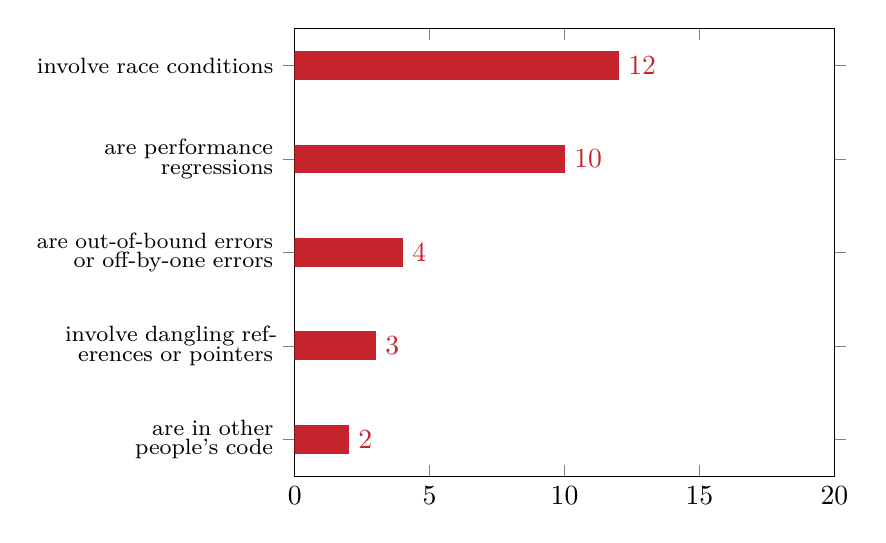
\begin{tikzpicture}
		\begin{axis}[
			results,
			symbolic y coords = {
				{are in other people's code},
				{involve dangling references or pointers},
				{are out-of-bound errors or off-by-one errors},
				{are performance regressions},
				{involve race conditions},
			}
		]
			\addplot coordinates {
				(12,{involve race conditions})
				(10,{are performance regressions})
				( 4,{are out-of-bound errors or off-by-one errors})
				( 3,{involve dangling references or pointers})
				( 2,{are in other people's code})
			};
		\end{axis}
	\end{tikzpicture}
	\caption{Answers of \gls{ssl} employees to the question \enquote{Most bugs I encounter\textellipsis} (\( N = 19 \)).}
	\label{fig:bugs}
\end{figure}

\section{Background}
Fortran (formerly FORTRAN) is the oldest of the programming languages we consider in this thesis. It was created in the 1950s at IBM by \citefullauthor{BackusFORTRANautomaticcoding1957}~\cite{BackusFORTRANautomaticcoding1957}, and featured the first optimizing compiler~\cite{PaduaFORTRANcompiler2000}. The first Fortran standard was published by \gls{ansi} in \citeyear{Fortran66}~\cite{Fortran66}, and revised in \citeyear{Fortran77}~\cite{Fortran77}. Further standards were published by \gls{iso} in \citeyear{Fortran90} (Fortran 90)~\cite{Fortran90}, \citeyear{Fortran95} (Fortran 95)~\cite{Fortran95}, \citeyear{Fortran2003} (Fortran 2003)~\cite{Fortran2003}, \citeyear{Fortran2008} (Fortran 2008)~\cite{Fortran2008} and \citeyear{Fortran2018}~\cite{Fortran2018}, adding support for free-form input, modules, dynamic memory allocation (Fortran 90); object-oriented programming (Fortran 2003); and co-arrays (Fortran 2008).

Compared to C++ and Rust, Fortran's defining features are its built-in support for multi-dimesional arrays, array slicing, and co-arrays. However, it lacks support for conditional compilation\footnote{most compilers support preprocessing using a C-like preprocessor. This is however not part of the Fortran standard.}, compile time-programming, inline assembly, and does not come with a standard library. Generic programming is supported, but not ergonomic. Compiler conformance varies strongly between vendors, with support for the newest standards being the least prevalent. It is not uncommon for compilers to provide their own extensions to alleviate percieved deficiencies of the standard.

\begin{listing}
	\centering
	\begin{minted}{fortran}
		program main
			print *, "Hello, World!"
		end program
	\end{minted}
	\caption{A \enquote{Hello, World!} program in Fortran.}
\end{listing}

C++ was developed in 1979 at AT\&T Bell Laboratories (now Nokia Bell Laboratories), by \citefullauthor{StroustrupProgrammingLanguage1985}. It was not made public until \citeyear{StroustrupProgrammingLanguage1985}, when \citetitle{StroustrupProgrammingLanguage1985} appeared. \gls{iso} standardised the language in \citeyear{Cpp98}~\cite{Cpp98}, and revised it in \citeyear{Cpp03}~\cite{Cpp03}. Since \citeyear{Cpp11}, the \gls{iso} C++ Standard follows a three-year release schedule \cites{Cpp11, Cpp14, Cpp17, Cpp20}.

C++ features support for the C preprocessor as a means of conditional compilation. C++11 added support for compile-time programming using \mintinline{c++}{constexpr}, with newer standards expanding the functionality. Templates provide support for generic functions and types, as well as allowing template meta-programming. Modern compilers adhere to the standard well, and conformance is tracked~\cite{CppCompilerSupport}.

\begin{listing}
	\centering
	\begin{minted}{c++}
		#include <iostream>

		int main() {
			std::cout << "Hello, World!" << std::endl;
		}
	\end{minted}
	\caption{A \enquote{Hello, World!} program in C++.}
\end{listing}

Rust is the youngest programming language of the three. Its development was started in 2006 at Mozilla Research by Graydon Hoare, with the version 1.0 being release in 2015. Since then, development has been taken over by the core team, with releases happening every 6 weeks.

Rust distinguishes itself from Fortran and C++ by bundling tooling with the compiler, allowing for easy dependency management, testing, and documentation generation. Much effort is put into making compiler messages clear and understandable: this includes providing suggestions for fixing code and path trimming~\cite{AloniPathTrimmingNightly2020}. Development of the language happens online, and is accessible to anyone interested, with the core team and community being open to contributions\footnote{Incidentaly, the author was able to successfully upstream a patch~\cite{SudwojNVPTXsupportnew2020} to the compiler, with guidance from the community.}. However, the Rust language and its reference compiler \texttt{rustc} are heavily intertwined. To date, no other compiler exists for Rust. Furthermore, Rust development is ongoing\textemdash{}it is by far not as mature of a language as Fortran or C++, as evidenced by the large amount of crucial features that are currently in development, such as constant functions, constant generics, specialization, generic associated types and support for GPU targets. On the other hand, being a young languge, Rust does away with a lot of the cruft of the past such as mutable-by-default variables, while allowing the programmer to opt-in to dangerous features when it is required\textemdash{}unsafe blocks limit such code to small small sections, whose contraints can easily be verified for soundness. Macros in Rust are hygienic, meaning that identifiers introduced in the macro will not \enquote{leak} or collide by chance with one declared by the user, as is the case in C and C++. The syntax of macros is also much more ergonomic: macros can be declared \enquote{by example}, with subsitiution placeholders for tokens when called. When more flexibility is needed, procedural macros can be written, which are Rust functions called at compile-time that transform the token stream. The Rust team take great care when extending the language and reference compiler, making sure that there are no regressions of runtime performance or compile-times, and scanning the whole public ecosystem before introducing breaking changes so as to assess the impact (in any case, automatic migration tools are provided with such changes).

\begin{listing}
	\centering
	\begin{minted}{rust}
		fn main() {
			println!("Hello, World!");
		}
	\end{minted}
	\caption{A \enquote{Hello, World!} program in Rust.}
\end{listing}

\section{Rust as a HPC programming language}
\todo{introductory paragraph}{}

Installing Rust is as easy as following the instructions on \url{rustup.rs}. The \texttt{rustup}~\cite{rustup} installer provides automatically generated binaries of the Rust toolchain; in addition, it allows us to install specific versions of Rust, extra targets and tools such as \texttt{rustfmt}~\cite{rustfmt}, the Rust code formatting utility.

Rust can also be installed from the operating system package manager (in case of Linux distributions), or from source using \texttt{spack}~\cite{spack}. However, we do not reccomend these approaches, as we consider the \texttt{rustup} installer to be superior. In comparision to a system package manager, it allows for installation of multiple versions of Rust, as well as arbitrary historical versions, should those be needed eg.\ to reproduce results from past studies. In comparision to \texttt{spack}, the \texttt{rustup} supports installation of arbitrary nightly versions of the toolchain\footnote{until 2020-09-08, support for installing extra targets, such as the NVIDIA GPGPU toolchain was also lacking in \texttt{spack}~\cite{SudwojRustaddednvptx}.}.

\begin{listing}
	\centering
	\begin{minted}{console}
		> curl --proto '=https' --tlsv1.2 -sSf https://sh.rustup.rs | sh
		> rustup toolchain install stable
		> rustup toolchain install nightly
		> rustup toolchain install nightly-2020-05-01
		> rustup target    install nvptx64-nvidia-cuda
	\end{minted}
	\caption{Example of installing \texttt{rustup} as well as different toolchains.}
\end{listing}

In terms of language and library features, Rust does not include support for complex numbers or multi-dimesional arrays out of the box. However, mature Rust libraries exist to support these features: \texttt{num-complex} for complex numbers; and \texttt{ndarray} and \texttt{nalgebra} for array and matrix support~\cite{num-complex,ndarray,nalgebra}. Bindings for BLAS and LAPACK are provided by the \texttt{blas}, \texttt{lapack}, \texttt{cblas}, \texttt{lapacke} crates~\cite{blas-lapack-rs}. A pure Rust implementation of general matrix multiplication is implemented in \texttt{matrixmultiply}~\cite{matrixmultiply}. MPI, HDF5 and netCDF are supported through the \texttt{mpi}, \texttt{hdf5} and \texttt{netcdf} crates, respectively, which are nearly feature-complete~\cite{mpi,hdf5,netcdf}. Bindings to other libraries can be generated in an automated manner using \texttt{bindgen}, while for the inverse case \texttt{cbindgen} can be used~\cite{bindgen,cbindgen}. \texttt{cxx} and \texttt{autocxx} provide additional features~\cite{cxx,autocxx}. Multi-threading and shared-memory parallelism is supported by the \texttt{rayon} crate, while \texttt{crossbeam} and \texttt{parking\_lot} provide optimized low-level synchronization primitives~\cite{rayon,crossbeam,parking-lot}.

We find Rust, and its ecosystem, to lack support for GPU programming, however. Firstly, there is currently no compiler backend support for AMD graphic cards, only for NVIDIA ones. Secondly, this support is only preliminary, and not automatically tested; calling a GPU kernel function or accessing the thread index requires unstable features, and therefore \texttt{nightly} Rust. Thirdly, most GPU code written in Rust will be \mintinline{rust}{unsafe} or even unsound, as the compiler cannot reason about the GPU memory model. Lastly, some performance-critical features, such as CUDA shared and constant memory, cannot be mapped to the current Rust memory model, and are therefore not implemented; we also doubt that they will be in the foreseeable future. Crates such as \texttt{rustacuda}, \texttt{ptx-builder}, \texttt{ptx-support} and \texttt{accel} do their best to provide as complete of a CUDA programming experience in Rust as possible~\cite{rustacuda,ptx-builder,ptx-support,accel}. A good overview of the current Rust ecosystems for machine learning, scientific computing and GPU offloading can be found at \url{https://www.arewelearningyet.com}~\cite{NowellArewelearning}.

In order to fully make use of Rust on a \gls{hpc} system, some environment variables might need to be set. For starters, certain crates might need help finding system libraries or tools, eg.\ \texttt{mpi} requires \mintinline{bash}{MPICC} to be set to the MPI C compiler wrapper, while \texttt{rustacuda} requires \mintinline{bash}{CUDA_LIBRARY_DIRECTORY} to locate the CUDA runtime libraries. Furthermore, code-generation options might need to be adjusted; if linking using the Cray toolchain on Piz Daint, we found that we had to set \mintinline{bash}{RUSTFLAGS="-C relocation-model=dynamic-no-pic"}. Lastly, in order to optimize for the underlying architecture, the target CPU should be specified, eg.\ \mintinline{bash}{RUSTFLAGS="-C target-cpu=haswell"}. The complete reccomended set of environment variables for Piz Daint can be found in \cref{lst:rustflags}.

\begin{listing}
	\centering
	\begin{minted}{console}
		> export CARGO_TARGET_X86_64_UNKNOWN_LINUX_GNU_RUSTFLAGS="-C target_cpu=${CRAY_CPU_TARGET:-haswell} -C relocation-model=dynamic-no-pic"
		> export CARGO_TARGET_NVPTX64_NVIDIA_CUDA_RUSTFLAGS="-C target-cpu=sm_60 -C target-feature=+sm_60,+ptx60 -C relocation-model=dynamic-no-pic"
		> export MPICC=cc
		> export CUDA_LIBRARY_PATH=${CUDATOOLKIT}/lib64
	\end{minted}
	\caption{The environment flags used on Piz Daint.}
	\label{lst:rustflags}
\end{listing}

% \clearpage
% \begin{todolist}
% 	\item Fortran
% 		\begin{itemize}
% 			\item developed in 1950s at IBM by John Backus
% 			\item first optimizing compiler
% 			\item first standardised in 1966 by ANSI, revised in 1977, 1990 (ISO), 1995, 2003, 2008, 2018
% 			\item Compilers: Gfortran, Flang, Intel, Cray, PGI, ...
% 			\item Codes: BLAS, LAPACK, cp2k, ...
% 		\end{itemize}
% 	\item C++
% 		\begin{itemize}
% 			\item developed in 1979 at AT\&T Bell Laboratories (now Nokia Bell Laboratories) by Bjarne Stroustrup
% 			\item publicised in 1985 in "The C++ Programming Language"
% 			\item standardised by ISO in 1998, revised in 2003, 2011, 2014, 2017, 2020
% 			\item follows 3 year release period
% 			\item Compilers: GCC, Clang, Intel, Cray, PGI, ...
% 			\item Codes: HPX, Eigen, BETL, ...
% 		\end{itemize}
% 	\item[\done] Rust
% 		\begin{itemize}
% 			\item developed in 2006 at Mozilla Research by Graydon Hoare
% 			\item first stable release (1.0) on (May 15) 2015
% 			\item reference compiler \texttt{rustc}, LLVM backend
% 			\item six-week release cycle
% 			\item good tooling (\texttt{cargo}, \texttt{rustup})
% 			\item open-source
% 			\item open-forum, online development of language
% 			\item Compilers: rustc, (cranelift)
% 			\item Code: rustsim.org, ndarray
% 		\end{itemize}
% 	\item GPU programming support
% \end{todolist}

\chapter{Performance}
\label{ch:performance}
\begin{displayquote}[\citefullauthor{KnuthStructuredProgramminggo1974}~\cite{KnuthStructuredProgramminggo1974}]
	Programmers waste enormous amounts of time thinking about, or worrying about, the speed of noncritical parts of their programs, and these attempts at efficiency actually have a strong negative impact when debugging and maintenance are considered. We \textbf{should} forget about small efficiencies, say about 97\% of the time: premature optimization is the root of all evil.

	Yet we should not pass up our opportunities in that critical 3\%.
\end{displayquote}

\section{Previous work}
We provide a short overview of the literature known to us that compares the performance of Rust to other languages.

\begin{itemize}
	\item \Citeauthor{Sverdrupgemmrabbithole2016} implemented matrix multiplication in Rust, being \slower{23\% slower than OpenBLAS}~\cite{Sverdrupgemmrabbithole2016, Sverdrupblussmatrixmultiply2020}
	\item \Citeauthor{WilkensEvaluationperformanceproductivity2015} compares C, Go and Rust implementations of Dijkstra's algorithm (finding the single-source shortest paths in a graph) in terms of productivity and performance~\cite{WilkensEvaluationperformanceproductivity2015}; finding the Rust implementation to be \faster{26\textendash50\% faster than C}, and \faster{7\textendash17\% faster than Go}, depending on the number of threads used.
	\item \citeauthor{PerezRustperformanceAlgorithmic2017} compares C++ and Rust implementations of the algorithmic Lovász Local Lemma (determining the probability that none of a set of event will occur, where each event is nearly independent from all others) in terms of productivity and performance~\cite{PerezRustperformanceAlgorithmic2017}; finding Rust to be \faster{43\textendash78\% faster than C++ in serial code}\footnote{Rust was also \faster{43\textendash{}78\% faster than C++ in parallel code}. However, the C++ parallel version was slower than the C++ serial version, with 60\% of time being spent creating and joining threads. This author presumes a thread pool was not used.}. % Crossbeam, std::thread
	\item \Citeauthor{McKeoghRewritingFORTRANSoftware2020} compares Fortran and Rust implementations of shallow-water equations~\cite{McKeoghRewritingFORTRANSoftware2020}(a system of hyperbolic partial differential equations, being an approximation to the Navier-Stokes equation, when the depth of the fluid is much smaller than the horizontal domain); finding Rust to be between \slower{59\% slower} and \faster{30\% faster} than Fortran, depending on problem size. % OpenMP, Rayon
	\item \Citeauthor{LindgrenComparingparallelRust2020} compares C++ and Rust performance of a constrained version of the all-pairs shortest paths problem from graph theory~\cite{LindgrenComparingparallelRust2020}; finding the final Rust version to be \slower{10\% slower} than the final C++ version\footnote{During the optimization process, Rust was between \slower{27\% slower} and \faster{18\% faster} than the corresponding C++ version.}.
	\item \Citeauthor{HahnOneProgramWritten2019} compares Python, Go and Rust implementations of \texttt{diffimg}, a tool for comparing images~\cite{HahnOneProgramWritten2019}; finding Rust to be \faster{35\textendash{}58\% faster than Go}, and \faster{65\textendash{}80\% faster than Python}, depending on problem size.
	\item \Citeauthor{Blanco-CuaresmaWhatcanprogramming2016} compare C, Fortran, Go, Julia and Rust implementations of a simple N-body physics simulation~\cite{Blanco-CuaresmaWhatcanprogramming2016, Blanco-Cuaresmamarblestationbenchmarkleapfrog2018}; finding Rust to be \faster{12\% faster than C}, \faster{22\% faster than Fortran}, \faster{36\% faster than Julia}, and \faster{39\% faster than Go}.
	\item \Citeauthor{AtchesonRustFloatingpointIntensive2019} compares C++ and Rust implementations of the generalized minimal residual method (an iterative method for finding the solution to a non-symmetric system of linear equations)~\cite{AtchesonRustFloatingpointIntensive2019}.
\end{itemize}

The above-mentioned works show that Rust achieve performance comparable to other languages under a variety of conditions; however, we find all the above references to be either to specialized to a specific problem, or to not offer a fair comparison, due to optimization deficiencies in implementation. In this thesis, we would like to show that that is also the case for numerical codes, as could be written by a domain scientist. To this end, we implement a stencil code as detailed in \cref{sec:background,sec:implementation} in Fortran, C++, and Rust.

% \Citeauthor{LesinskiSpeedRustvs} compares C and Rust in terms of features and overheads~\cite{LesinskiSpeedRustvs};

\section{Background}
\label{sec:background}
\begin{displayquote}[\citefullauthor{TrefethenFiniteDifferenceSpectral1996}~\cite{TrefethenFiniteDifferenceSpectral1996}]
	Finite difference approximations have a more complicated \enquote{physics} than the equations they are designed to simulate. This irony is no paradox, however, for finite differences are used not because the numbers they generate have simple properties, but because those numbers are simple to compute.
\end{displayquote}

As a basis for our language comparison, we choose the fourth-order numerical diffusion equation in the \( xy \)-plane,
\begin{equation}
	\pdv{\phi}{t} =
		-\alpha_{4} \nabla^{4} \phi =
		-\alpha_{4} \laplacian^{2} \phi =
		-\alpha_{4} \laplacian (\laplacian \phi), \label{eq:4th-order-diffusion}
\end{equation}
where \( \phi \) is a scalar-valued function of space and time. Such an equation could be eg.\ used as a noise filter in a climate or weather simulation~\cite{XueHighordermonotonicnumerical2000}. More importantly, we discretize this equation using finite differences, which are abundantly used in scientific codes, and which leads us to believe that this is a suitable benchmark.

We solve \cref{eq:4th-order-diffusion} on a cubic grid. Choosing a uniform spatial discretization in the horizontal plane and time, and an arbitrary discretization in the vertical direction, we define
\begin{equation}
	\phi_{i, j, k}^{n} \stackrel{\mathrm{def}}{\approx} \phi(x_{i}, y_{j}, z_{k}, t^{n})
\end{equation}
to be the approxiamte value of the function at the grid points
\begin{subequations}
	\begin{align}
		x_{i} &\stackrel{\mathrm{def}}{=} i \cdot \increment x &\text{where } &1 \leq i \leq n_{x}, \\
		y_{j} &\stackrel{\mathrm{def}}{=} j \cdot \increment y &\text{where } &1 \leq j \leq n_{y}, \\
		z_{k} &\stackrel{\mathrm{def}}{=} z(k)                 &\text{where } &1 \leq k \leq n_{z} \text{ and} \\
		t^{n} &\stackrel{\mathrm{def}}{=} n \cdot \increment t &\text{where } &1 \leq n \leq T.
	\end{align}
\end{subequations}
We then approximate the laplacian using a second-order central finite difference,
\begin{equation}
	\laplacian \phi_{i, j, k}^{n} \approx
		\frac{-4 \phi_{i, j, k}^{n} + \phi_{i - 1, j, k}^{n} + \phi_{i + 1, j, k}^{n} + \phi_{i, j - 1, k}^{n} + \phi_{i, j + 1, k}^{n}}{\increment x \increment y}.
\end{equation}
For the time derivative, we use a first-order forward difference (explicit Euler method),
\begin{equation}
	\pdv{\phi_{i, j, k}^{n}}{t} \approx \frac{\phi_{i, j, k}^{n + 1} - \phi_{i, j, k}^{n}}{\increment t}.
\end{equation}
Solving for $\phi_{i, j, k}^{n + 1}$, we get the following finite difference scheme,
\begin{subequations}
	\begin{align}
		\psi_{i, j, k}^{n} &=
			\frac{1}{\increment x \increment y} \left(
				-4 \phi_{i,     j,     k}^{n}
				+  \phi_{i - 1, j,     k}^{n}
				+  \phi_{i + 1, j,     k}^{n}
				+  \phi_{i,     j - 1, k}^{n}
				+  \phi_{i,     j + 1, k}^{n}
			\right) \label{eq:laplap1} \\
		\phi_{i, j, k}^{n + 1} &=
			\phi_{i, j, k}^{n} - \frac{\alpha_{4} \increment t}{\increment x \increment y} \laplacian \left(
				-4 \psi_{i,     j,     k}^{n}
				+  \psi_{i - 1, j,     k}^{n}
				+  \psi_{i + 1, j,     k}^{n}
				+  \psi_{i,     j - 1, k}^{n}
				+  \psi_{i,     j + 1, k}^{n}
			\right), \label{eq:laplap2}
	\end{align}
\end{subequations}
which can be further simplified to
\begin{equation}
	\begin{aligned}
	\phi_{i, j, k}^{n + 1} =
		\phi_{i, j, k}^{n} - \frac{\alpha_{4} \increment t}{(\increment x)^{2} (\increment y)^{2}} \left( \vphantom{\phi_{i, j, k}^{n}} \right.
			& -20 \phi_{i,     j,     k}^{n} \\
			& + 8 \phi_{i - 1, j,     k}^{n}
			  + 8 \phi_{i + 1, j,     k}^{n}
			  + 8 \phi_{i,     j - 1, k}^{n}
			  + 8 \phi_{i,     j + 1, k}^{n} \\
			& - 2 \phi_{i - 1, j - 1, k}^{n}
			  - 2 \phi_{i - 1, j + 1, k}^{n}
			  - 2 \phi_{i + 1, j - 1, k}^{n}
			  - 2 \phi_{i + 1, j + 1, k}^{n} \\
			& -   \phi_{i - 2, j,     k}^{n}
			  -   \phi_{i + 2, j,     k}^{n}
			  -   \phi_{i,     j - 2, k}^{n}
			  -   \phi_{i,     j + 2, k}^{n}
		  \left. \vphantom{\phi_{i, j, k}^{n}} \right)
	\end{aligned} . \label{eq:inline}
\end{equation}
\Cref{eq:laplap1,eq:laplap2} can be expressed as the stencil shown in \cref{fig:laplap}, while \cref{eq:inline} gives rise to the stencil in \cref{fig:inline}.

\begin{figure}
	\centering
	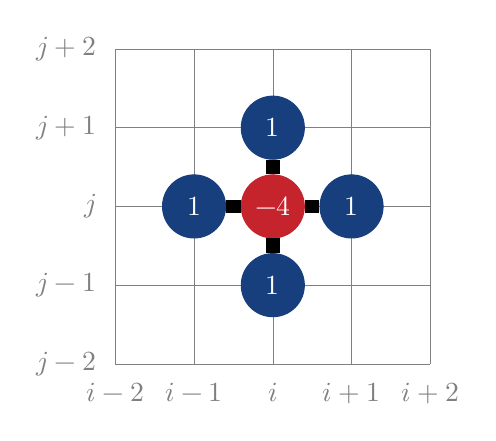
\begin{tikzpicture}
		\begin{scope}[help lines]
			\draw (-2, -2) grid (+2, +2);

			\node at (-2, -2) [label = below:$i - 2$] {};
			\node at (-1, -2) [label = below:$i - 1$] {};
			\node at ( 0, -2) [label = below:$i$]     {};
			\node at (+1, -2) [label = below:$i + 1$] {};
			\node at (+2, -2) [label = below:$i + 2$] {};

			\node at (-2, -2) [label = left:$j - 2$] {};
			\node at (-2, -1) [label = left:$j - 1$] {};
			\node at (-2,  0) [label = left:$j$]     {};
			\node at (-2, +1) [label = left:$j + 1$] {};
			\node at (-2, +2) [label = left:$j + 2$] {};
		\end{scope}

		\begin{scope}[
			every node/.style = {
				circle,
				inner sep = 0pt,
				minimum size = 0.8cm,
				text = white,
			},
		]
			\node at ( 0,  0) [draw = ETHRed,      fill = ETHRed]      (ij)   {$-4$};
			\node at (-1,  0) [draw = ETHDarkBlue, fill = ETHDarkBlue] (i-1j) {$ 1$};
			\node at (+1,  0) [draw = ETHDarkBlue, fill = ETHDarkBlue] (i+1j) {$ 1$};
			\node at ( 0, -1) [draw = ETHDarkBlue, fill = ETHDarkBlue] (ij-1) {$ 1$};
			\node at ( 0, +1) [draw = ETHDarkBlue, fill = ETHDarkBlue] (ij+1) {$ 1$};
		\end{scope}

		\draw[line width = 5pt]
			(ij) -- (i-1j)
			(ij) -- (i+1j)
			(ij) -- (ij-1)
			(ij) -- (ij+1)
		;
	\end{tikzpicture}
	\caption{Five-point stencil used in \texttt{laplap}.}
	\label{fig:laplap}
\end{figure}

\begin{figure}
	\centering
	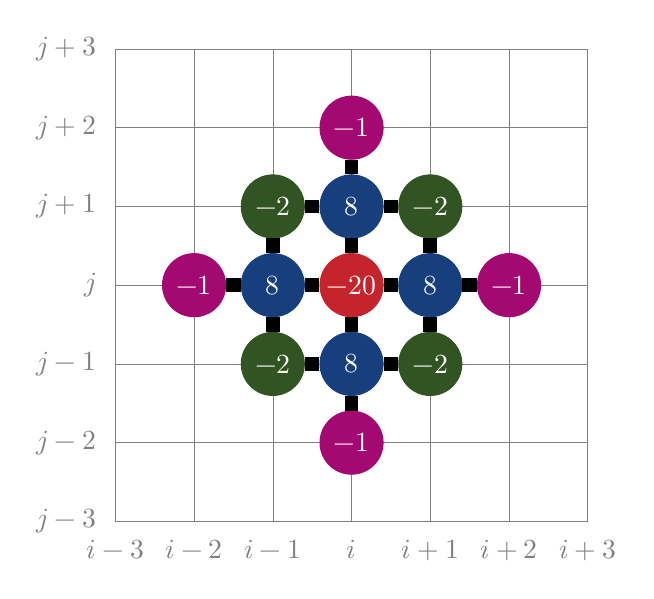
\begin{tikzpicture}
		\begin{scope}[help lines]
			\draw (-3, -3) grid (+3, +3);
			\node at (-3, -3) [label = left:$j - 3$] {};
			\node at (-3, -2) [label = left:$j - 2$] {};
			\node at (-3, -1) [label = left:$j - 1$] {};
			\node at (-3,  0) [label = left:$j    $] {};
			\node at (-3, +1) [label = left:$j + 1$] {};
			\node at (-3, +2) [label = left:$j + 2$] {};
			\node at (-3, +3) [label = left:$j + 3$] {};

			\node at (-3, -3) [label = below:$i - 3$] {};
			\node at (-2, -3) [label = below:$i - 2$] {};
			\node at (-1, -3) [label = below:$i - 1$] {};
			\node at ( 0, -3) [label = below:$i    $] {};
			\node at (+1, -3) [label = below:$i + 1$] {};
			\node at (+2, -3) [label = below:$i + 2$] {};
			\node at (+3, -3) [label = below:$i + 3$] {};
		\end{scope}

		\begin{scope}[
			every node/.style = {
				circle,
				inner sep = 0pt,
				minimum size = 0.8cm,
				text = white,
			},
		]
			\node at ( 0,  0) [draw = ETHRed,       fill = ETHRed]       (ij)     {$-20$};
			\node at (-1,  0) [draw = ETHDarkBlue,  fill = ETHDarkBlue]  (i-1j)   {$  8$};
			\node at (+1,  0) [draw = ETHDarkBlue,  fill = ETHDarkBlue]  (i+1j)   {$  8$};
			\node at ( 0, -1) [draw = ETHDarkBlue,  fill = ETHDarkBlue]  (ij-1)   {$  8$};
			\node at ( 0, +1) [draw = ETHDarkBlue,  fill = ETHDarkBlue]  (ij+1)   {$  8$};
			\node at (-1, -1) [draw = ETHDarkGreen, fill = ETHDarkGreen] (i-1j-1) {$- 2$};
			\node at (-1, +1) [draw = ETHDarkGreen, fill = ETHDarkGreen] (i-1j+1) {$- 2$};
			\node at (+1, -1) [draw = ETHDarkGreen, fill = ETHDarkGreen] (i+1j-1) {$- 2$};
			\node at (+1, +1) [draw = ETHDarkGreen, fill = ETHDarkGreen] (i+1j+1) {$- 2$};
			\node at (-2,  0) [draw = ETHMagenta,   fill = ETHMagenta]   (i-2j)   {$- 1$};
			\node at (+2,  0) [draw = ETHMagenta,   fill = ETHMagenta]   (i+2j)   {$- 1$};
			\node at ( 0, -2) [draw = ETHMagenta,   fill = ETHMagenta]   (ij-2)   {$- 1$};
			\node at ( 0, +2) [draw = ETHMagenta,   fill = ETHMagenta]   (ij+2)   {$- 1$};
		\end{scope}

		\draw[line width = 5pt]
			(ij)   -- (i-1j)
			(ij)   -- (i+1j)
			(ij)   -- (ij-1)
			(ij)   -- (ij+1)
			(i-1j) -- (i-1j-1)
			(i-1j) -- (i-1j+1)
			(i-1j) -- (i-2j)
			(i+1j) -- (i+1j-1)
			(i+1j) -- (i+1j+1)
			(i+1j) -- (i+2j)
			(ij-1) -- (i-1j-1)
			(ij-1) -- (i+1j-1)
			(ij-1) -- (ij-2)
			(ij+1) -- (i-1j+1)
			(ij+1) -- (i+1j+1)
			(ij+1) -- (ij+2)
		;
	\end{tikzpicture}
	\caption{Thirteen-point stencil used in \texttt{inline}.}
	\label{fig:inline}
\end{figure}

For ease of implementation, we define \( \alpha \stackrel{\mathrm{def}}{=} \alpha_4 (\increment t) (\increment x)^{-2} (\increment y)^{-2} \); this can be interpreted as \( \increment t = \increment x = \increment y = 1 \). In order for the schemes to be stable, \( \alpha \) must satisfy the CFL condition; we assume this is the case, and choose an appropriately small \( \alpha \) for all our experiments.

Implementing \cref{eq:laplap1,eq:laplap2} in code results in \cref{alg:laplap}, which we name \textbf{\texttt{laplap}}. We note that this scheme requires a temporary array of size \( n_{x} \cdot n_{y} \). In turn \cref{eq:inline} results in \cref{alg:inline}, which we name \textbf{\texttt{inline}}.

\begin{algorithm}
	\For{$n \leftarrow 1$ \KwTo $T$}{
		\For{$k \leftarrow 1$ \KwTo $n_{z}$}{
			\For{$j \leftarrow 1$ \KwTo $n_{y}$}{
				\For{$i \leftarrow 1$ \KwTo $n_{x}$}{$
					\mathtt{tmp}_{i, j} \leftarrow
						-4 \cdot \mathtt{in}_{i,     j,     k}
						+        \mathtt{in}_{i - 1, j,     k}
						+        \mathtt{in}_{i + 1, j,     k}
						+        \mathtt{in}_{i,     j - 1, k}
						+        \mathtt{in}_{i,     j + 1, k}
				$\;}
			}

			\For{$j \leftarrow 1$ \KwTo $n_{y}$}{
				\For{$i \leftarrow 1$ \KwTo $n_{x}$}{
					$
						\mathtt{laplap} \leftarrow
							-4 \cdot \mathtt{tmp}_{i,     j}
							+        \mathtt{tmp}_{i - 1, j}
							+        \mathtt{tmp}_{i + 1, j}
							+        \mathtt{tmp}_{i,     j - 1}
							+        \mathtt{tmp}_{i,     j + 1}
					$\;
					\uIf{$n = T$}{$
						\mathtt{out}_{i, j, k} \leftarrow \mathtt{in}_{i, j, k} - \alpha \cdot \mathtt{laplap}
					$\;}
					\Else{$
						\mathtt{in}_{i, j, k} \leftarrow \mathtt{in}_{i, j, k} - \alpha \cdot \mathtt{laplap}
					$\;}
				}
			}
		}
	}
	\caption{The \texttt{laplap} algorithm.}
	\label{alg:laplap}
\end{algorithm}

\begin{algorithm}
	\For{$n \leftarrow 1$ \KwTo $T$}{
		\For{$k \leftarrow 1$ \KwTo $n_{z}$}{
			\For{$j \leftarrow 1$ \KwTo $n_{y}$}{
				\For{$i \leftarrow 1$ \KwTo $n_{x}$}{$
					\mathtt{out}_{i, j, k} \leftarrow
						(-20 \alpha + 1) \cdot \mathtt{in}_{i,     j,     k}
						 + 8 \alpha      \cdot \mathtt{in}_{i - 1, j,     k}
						 + 8 \alpha      \cdot \mathtt{in}_{i + 1, j,     k}
						 + 8 \alpha      \cdot \mathtt{in}_{i,     j - 1, k}
						 + 8 \alpha      \cdot \mathtt{in}_{i,     j + 1, k}
						 - 2 \alpha      \cdot \mathtt{in}_{i - 1, j - 1, k}
						 - 2 \alpha      \cdot \mathtt{in}_{i - 1, j + 1, k}
						 - 2 \alpha      \cdot \mathtt{in}_{i + 1, j - 1, k}
						 - 2 \alpha      \cdot \mathtt{in}_{i + 1, j - 1, k}
						 -   \alpha      \cdot \mathtt{in}_{i - 2, j,     k}
						 -   \alpha      \cdot \mathtt{in}_{i + 2, j,     k}
						 -   \alpha      \cdot \mathtt{in}_{i,     j - 2, k}
						 -   \alpha      \cdot \mathtt{in}_{i,     j + 2, k}
				$\;}
			}
		}
		\If{$n \neq T$}{$
			\mathtt{swap}(\mathtt{in}, \mathtt{out})
		$\;}
	}
	\caption{The \texttt{inline} algorithm.}
	\label{alg:inline}
\end{algorithm}

% for laplap algorithm:
% laplap: 5 mul, 4 add, 6 ld/st (3H, 3M)
% tmp1_field -> (nx + 2 * num_halo - 2) * (ny + 2 * num_halo - 2) * nz
% laplap -> nx * ny * nz
% final store: 1 mul, 1 add, 2ld/st (1H 1M, unless last iteration, then 2M)


% \begin{Theorem}[Amdahl's Law] % Strong scaling
% 	\[ S_{p} = \frac{1}{f + \frac{1 - f}{p}} \]
% \end{Theorem}
% 
% \begin{Theorem}[Gustafsson's Law] % Weak scaling
% 	\[ S_{p} = f + p (1 - f) \]
% \end{Theorem}

\section{Implementation}
\label{sec:implementation}
The author implemented \cref{alg:laplap,alg:inline} in Fortran, C++ and Rust. The author considers himself to be a novice Fortran programmer, an advanced C++ programmer and an average Rust programmer, having about 4 weeks, 5 years and 1 year of experience in each respectively.

In addition to the sequential version in each langauge, we implemented the following versions: in Fortran, using OpenMP, OpenMP offloading, OpenACC, and CUDA; in C++, using OpenMP, OpenMP offloading, OpenACC, and CUDA; and in Rust using \texttt{rayon}, \texttt{accel}, and CUDA. Complier support for these technologies varied, which we show in \cref{tab:fortran-support,tab:cpp-support,tab:rust-support}. We used optimization reports from compilers to confirm that code was being vectorized and offloaded where desired, and used flamegraphs~\cite{Greggflamegraph2016}\todo{add figure if available, explain how they help (inling, \% function time)}{} and CrayPat reports to check that out code was optimized; in cases where it was not, we implemented further optimizations by hand, as described in \cref{sec:results}.

\begin{table}
	\centering
	\begin{threeparttable}
		\begin{tabular}{ *{5}{l} }
			\toprule
			Technology
				&Cray (classic)
				&GNU
				&Intel
				&PGI
			\\
			\midrule
			OpenMP
				&\yes
				&\yes
				&\yes
				&\yes
			\\
			OpenMP offloading
				&\no[1]
				&\no[2]
				&\no
				&\yes
			\\
			OpenACC
				&\no[1]
				&\no[2]
				&\no
				&\runtimeerror[3]
			\\
			CUDA
				&\no
				&\no
				&\no
				&\yes
			\\
			\bottomrule
		\end{tabular}
		\begin{tablenotes}
			\makeatletter
			\footnotesize
			\item[\@fnsymbol{1}]{CUDA symbol not found}
			\item[\@fnsymbol{2}]{compiler compiled without offloading support}
			\item[\@fnsymbol{3}]{segmentation fault}
			\makeatother
		\end{tablenotes}
	\end{threeparttable}
	\caption{Fortran compiler support for different technologies.}
	\label{tab:fortran-support}
\end{table}

\begin{table}
	\centering
	\begin{threeparttable}
		\begin{tabular}{ *{5}{l} }
			\toprule
			Technology
				&Cray (\texttt{clang})
				&GNU
				&Intel
				&PGI
			\\
			\midrule
			OpenMP
				&\yes
				&\yes
				&\yes
				&\yes
			\\
			OpenMP offloading
				&\no[4]
				&\no[2]
				&\no
				&\yes
			\\
			OpenACC
				&\no
				&\no[2]
				&\no
				&\runtimeerror[5]
			\\
			CUDA (\texttt{nvcc})
				&\runtimeerror[6]
				&\yes
				&\runtimeerror[6]
				&\runtimeerror[7]
			\\
			\bottomrule
		\end{tabular}
		\begin{tablenotes}
			\makeatletter
			\footnotesize
			\item[\@fnsymbol{2}]{compiler compiled without offloading support}
			\item[\@fnsymbol{3}]{segmentation fault}
			\item[\@fnsymbol{4}]{CUDA invalid source}
			\item[\@fnsymbol{5}]{Invalid handle}
			\item[\@fnsymbol{6}]{CUDA invalid configuration}
			\item[\@fnsymbol{7}]{\texttt{ldd} could not find symbol}
			\makeatother
		\end{tablenotes}
	\end{threeparttable}
	\caption{C++ compiler support for different technologies.}
	\label{tab:cpp-support}
\end{table}

\begin{table}
	\centering
	\def\TPTminimum{\textwidth}
	\begin{threeparttable}
		\makebox[\linewidth]{
		\begin{tabular}{ *{2}{l} }
			\toprule
			Technology &\texttt{rustc} \\
			\midrule
			\texttt{rayon} &\yes \\
			\texttt{accel} &\yes[8] \\
			CUDA           &\no[9] \\
			\bottomrule
		\end{tabular}
		}
		\begin{tablenotes}
			\makeatletter
			\footnotesize
			\item[\@fnsymbol{8}]{using Rust version \texttt{nightly-2020-05-01} for device code}
			\item[\@fnsymbol{9}]{could not compile dependencies}
			\makeatother
		\end{tablenotes}
	\end{threeparttable}
	\caption{Rust compiler support for different technologies.}
	\label{tab:rust-support}
\end{table}

\section{Setup}
\label{sec:setup}
We compiled the C++ and Fortran implementations using the four available toolchains on Piz Daint: Cray, GNU, Intel and PGI. The Rust implementation was compiled using the reference Rust compiler, \texttt{rustc}\footnote{For exact versions, see \cref{app:reproducibility}.}. CUDA C++ versions used the NVIDIA CUDA compiler for device code compilation. We used appropriate optimization flags specific to each compiler to generate optimized code. Link-time optimization was not enabled. However, Fortran and C++ code was compiled with non-associative floating-point operations enabled (\texttt{-ffast-math} or equivalent), while Rust code was not; instead, we wrote a version in Rust using a special floating-point type that only enables such optimizations locally. \Cref{sec:implementation} details the optmization process we undertook. All matrices were stored in column-major order, whose elements were single-precision floating-point numbers.

When parallelizing the code, care was taken to primarily split along the \( z \)-axis. While this might seem an artificial limitation for this simple code, it is more representative of a real-world scenario, where eg.\ in a climate code, many more operation and calculations would be performed for each vertical slice. Additionally, all artificial synchronization barriers were put at the end of each time iteration, as that is where inter-node communication would take place in a cluster-distributed simulation. This was left out due to time constraints, as it was deemed to be more dependent on the underlying vendor-provided communication library, rather than on any language itself.

The benchmark driver was written in Rust, and linked dynamically to each of the libraries containing the implementations. The initial conditions,
\begin{equation}
	\phi(x, y, z, 0) = \phi_{0}(x, y, z) = \begin{cases}
		1 \text{ if } 0.25 \leq x, y, z \leq 0.75 \\
		0 \text{ otherwise}
	\end{cases},
	\label{eq:initial-conditons}
\end{equation}
were set by the driver. A visualization thereof can be seen in \cref{fig:initial-conditions}. For ease of implementation, we used a hardwall boundary condition, fixing the value at the boundary to be \( 0 \). Additionally, the driver calculated the \( \mathcal{l}_{\infty} \)-error from the baseline for each measurement. This baseline was chosen to be the numerical solution to the problem as calculated by the sequential Fortran \texttt{laplap} version compiled using the Cray toolchain. During testing and debugging, we noticed that the error correlates strongly with the choice of algorithm and the number of iterations, being of the order of \num{1.5e-7} per iteration. We therefore conjecture that the main cause of error are floating-point associativity caused by algorithmic differences. Furthermore, parallel versions exhibited a slightly higher error of about \num{2e-7} per iteration, which is still in the precision range for single-precision floating-point arithmetic (6\textendash{}9 decimal digits). We verified that solutions were reasonable in all cases using graphical comparision. In the end, we set the threshold for accepting a solution as correct to be \num{2.5e-4} after 1024 iterations; all implementations fulfilled this criterion.

\begin{figure}
	\centering
	{\sffamily
		\input{initial_conditions}
	}
	\caption{Initial conditions and solution after 1024 iterations at \( z = 0.5 \).}
	\label{fig:initial-conditions}
\end{figure}

All code and measurement data are committed to to a version control system, and is available from the author upon request.

We ran the benchmark on Cray XC50 nodes of Piz Daint. Each of these consists of one Intel Xeon E5-2690v3 CPU and one Nvidia Tesla P100 GPU. \( \alpha \) was set to \( 0.03125 \) and the number of iterations was fixed at \( 1024 \). Note, that this means, that for higher resolution, the simulation was run for a shorter amount of physical time, in order to satisfy the CFL condition. Due to time constraints, we only ran the benchmarks once per language-compiler-version combination, but are confident that our results are consistent, due to them exhibiting consistency during testing and debugging.

\section{Results}
\label{sec:results}
\todo{code samples}{}
In this section, we present our findings. Out of the 84 language-compiler-algorithm-version combinations, 52 could be successfully benchmarked, as detailed in \cref{sec:implementation}. This resulted in 524 measurements, as CPU-parallelized versions were run on 1, 2, 4, 8 and 12 cores, so that a scaling analysis could be done\textemdash{}these are detailed in \cref{app:data}. Next to a discussion of the runtime measurements, we choose to provide a subjective, developer-diary-like description of our experience in working with each language and technology. \Cref{fig:scaling-seq,fig:scaling-cpu,fig:scaling-gpu} show the benchmark runtimes as functions of the problem size, algorithm, implementation language, compiler and technology used. Immediately, we see that all these factors affect the runtime, including the choice of algorithm.

For the sequential case, as shown in \cref{fig:scaling-seq}, we see that there is little difference between compilers for the majority of cases. Seemingly, only the Fortran PGI \texttt{laplap} version, the C++ PGI \texttt{inline}, and the Fortran GNU versions perform significantly worse. Our original Rust version, \texttt{seq}, also runs slower\textemdash{}this is unsurprising, as this direct translation from Fortran does an index bounds check on each array element access. The other Rust versions all perform comparatively fast; this includes using unchecked array element access (\texttt{seq\_unchecked}), explicitly using fused-multiply-add intrinsics (\texttt{seq\_fma}), non-associative floating-point operations (\texttt{seq\_fast}), and iterators (\texttt{seq\_zip}); this can be seen in \cref{fig:scaling-seq-rust} in more detail. Seeing this, we concluded that these approaches were all similarly performant, and chose not to implement the \texttt{fma} and \texttt{fast} versions in parallelized or offloaded code.

In terms of implementation effort, programming in Fortran was the most simple, due to language support for multi-dimensional arrays; however, error handling, such as asserting preconditions, was significantly more difficult, due to lack of a standard library. In the C++ implementation, we chose to write a simple array wrapper class; this was a simple enough task. Some compilers required annotating loops with directives, so that the code would be appropriately vectorized. Our Rust code ended up being most complicated. We used the \texttt{ndarray} crate for array support, deciding against \texttt{nalgebra} due to its lack of support for arrays of more than 2 dimensions. Translating simple loops from Fortran resulted in bad performance, due to bound-checking being performed on each access. This was to be expected. Using unchecked accesses required using \mintinline{rust}{unsafe} blocks, which we found to be bad practice. The iterator version (\texttt{seq\_zip}) was simliarly fast; however required naming each summand in \cref{eq:laplap1,eq:laplap2,eq:inline} separately, which we found to not be very ergonomical. Additionally, in the \texttt{inline} version, the \texttt{ndarray} crate had to be patched in order support higher arity of the \mintinline{rust}{zip!} macro. This also had to be done for the respective CPU versions.

\begin{figure}
	\centering
	{\sffamily
		\input{scaling_seq}
	}
	\caption{Scaling by size of the sequential versions.}
	\label{fig:scaling-seq}
\end{figure}

\begin{figure}
	\centering
	{\sffamily
		\input{scaling_seq_rust}
	}
	\caption{Scaling by problem size of the sequential Rust versions (detailed).}
	\label{fig:scaling-seq-rust}
\end{figure}

In the parallelized CPU versions, we see even more differences between compilers. The Intel C++ compiler produces the fastest running code. Surprisingly, the Rust \texttt{laplap} code using \texttt{rayon} parallel iterators (\texttt{par\_axis\_zip}) comes in second place, only about 20\% slower than the Intel version. Other compiler-language-algorithm combinations are significantly slower, by between 3.6x to 16.5x compared to the Rust version. Finally, the Intel Fortran compiler performs the worst, taking about 29 times as long to compute the solution, as the Intel C++ version. Due to time contraints, we were not able to fully analyze the issue, and are not sure how this discrepancy comes to be. We conjecture that given more time, we could significantly improve the time-to-solution of these versions, and bring them inline and closer to the others.

Implementation in Fortran and C++ was straightforward, being limited to the addition of OpenMP directives, barring minor non-adherence to the OpenMP standard in case of the GNU compiler; this was due to the version of the GNU toolchain that was available on the computing cluster\textemdash{}the issue has been resolved in GCC 9. On the Rust side, parallelization of code was similarly simple, by changing from a loop over all \( z \)-levels to using a parallel iterator over the \( z \)-axis.

All of our OpenMP implementations are parallelized only in the \( z \)-dimension; however, due to an error, our initial Rust implementation (labeled \texttt{par\_zip}), may parallelize over all dimensions; this issue was fixed in the \texttt{par\_axis\_zip} version. This artificial limitation is more representative of how a real climate code might be structured\textemdash{}nevertheless, we decided to include the \texttt{par\_zip} version in our results, because its scaling behaviour resembles that of the C++ versions compiled using the Intel toolchain. We hypothesize that the Intel C++ compiler might be optimizing our code more than we would want it to, as discusssed in \cref{sec:setup}.

\begin{figure}
	\centering
	{\sffamily
		\input{scaling_cpu}
	}
	\caption{Scaling by problem size of the parallelized versions (run on 12 cores).}
	\label{fig:scaling-cpu}
\end{figure}

As mentioned in \cref{sec:implementation}, and indicated by \cref{tab:fortran-support,tab:cpp-support}, we implemented offloading to the GPU in Fortran and C++ using OpenMP, OpenACC and CUDA. Sadly, it turned out that compiler support for these technologies was highly lacking. The Intel compiler used did not support any offloading to GPUs, only to Intel Xeon Phi coprocessors. The Cray-provided GNU toolchain was not compiled with offloading support; at the time of benchmarking, installation of a offloading-capable GNU compiler using \texttt{spack} resulted in errors during its building, as did the LLVM toolchain. The newer Cray-\texttt{clang} toolchain does not yet support OpenACC; while using OpenMP \texttt{target} directives with it resulted in seemingly invalid PTX code. The Cray-classic toolchain used for Fortran generated OpenMP-offloaded code that failed at runtime. CUDA device code generated by the NVIDIA \texttt{nvcc} compiler resulted in runtime errors in all cases except when linking to GNU-generated host code. In the end, out of the 17 officially supported configurations with Fortran and C++, we could only successfully benchmark 4.

While using Rust to generate GPU device code, we could not get our pure Rust implementation to work; it failed to create correct shared libraries for some dependencies; generating Rust libraries (\texttt{rlib}s) by hand worked, was however not compatible with our benchmark driver. Therefore, we could only benchmark the Rust version implemented using \texttt{accel}, which hardcodes the device compiler to be the Rust nightly version from 2020-05-01.

We see that in the case of GPU offloaded code, the Rust version is about 2x slower than some of the OpenMP offloaded versions. The CUDA Fortran and C++ versions are also slower than the OpenMP versions; we suspect this is due to us not using shared memory to optimize GPU memory accesses in our CUDA codes. This was not done on the one hand due to time constraints, on the other hand, to offer a fair comparison with Rust, which supports neither constant nor shared CUDA memory spaces.

The OpenMP-offloaded versions necessitated only small adjustments from multi-threaded OpenMP implementations. The OpenACC versions were in turn similar to these, due to the relatively small difference in the standards from end-user perspective. However, we were very dissappointed that none of the OpenACC versions could be successfully benchmarked. Furthermore, each toolchain implements such offloading in a different manner: the Cray-classic toolchain seems to create a shared library with only host code, loading and just-in-time-compiling device code at runtime; meanwhile, the PGI toolchain directly embeds the PTX and fatbin artefacts in the shared library. In all cases, we find the documentation to be very lacking in terms of instruction how to debug obscure errors seemingly related to the launching of OpenACC and OpenMP kernels; we are similarly dissapponted that these errors are not raised at compile-time. We had not expected that linking \texttt{nvcc}-compiled CUDA code with host code would be so cumbersome and error-ridden. However, we were pleasantly surprised at the ergonomics of CUDA Fortran\textemdash{}especially the use of custom attributes to designate host and device variables, and the implicit copying using the assignment operator between them.

Knowing that Rust support for GPU programming is in only experimentally supported, we did not have high expectations. We were mildly surprised in how \texttt{accel} provided a similar experience to CUDA C++; launching kernels from \texttt{accel} is a bit more explicit, however, as it required manual device selection and context creation. Due to Rust's safety guarantees, device code is inherently \mintinline{rust}{unsafe}; the pointer arithmetic is similar to CUDA C++, but does not feel very \emph{Rust-ic}. Our pure Rust implementation failed to fully compile (see \cref{tab:rust-support})\textemdash{}in our opinion this demonstrates the experimental state of GPU programming in Rust.

\begin{figure}
	\centering
	{\sffamily
		% Created by tikzDevice version 0.12.3.1 on 2022-05-06 17:52:49
% !TEX encoding = UTF-8 Unicode
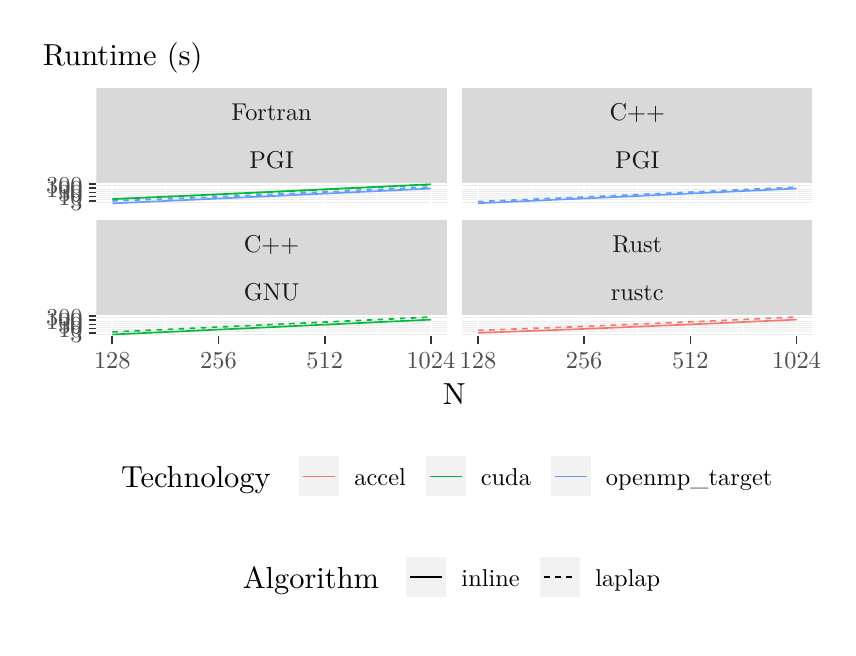
\begin{tikzpicture}[x=1pt,y=1pt]
\definecolor{fillColor}{RGB}{255,255,255}
\path[use as bounding box,fill=fillColor] (0,0) rectangle (289.08,216.81);
\begin{scope}
\path[clip] (  0.00,  0.00) rectangle (289.08,216.81);
\definecolor{drawColor}{RGB}{255,255,255}

\path[draw=drawColor,line width= 0.6pt,line join=round,line cap=round,fill=fillColor] (  0.00,  0.00) rectangle (289.08,216.81);
\end{scope}
\begin{scope}
\path[clip] ( 24.82,152.96) rectangle (151.45,160.55);
\definecolor{fillColor}{gray}{0.92}

\path[fill=fillColor] ( 24.82,152.96) rectangle (151.45,160.55);
\definecolor{drawColor}{RGB}{255,255,255}

\path[draw=drawColor,line width= 0.3pt,line join=round] ( 24.82,153.44) --
	(151.45,153.44);

\path[draw=drawColor,line width= 0.3pt,line join=round] ( 24.82,155.01) --
	(151.45,155.01);

\path[draw=drawColor,line width= 0.3pt,line join=round] ( 24.82,156.52) --
	(151.45,156.52);

\path[draw=drawColor,line width= 0.3pt,line join=round] ( 24.82,158.02) --
	(151.45,158.02);

\path[draw=drawColor,line width= 0.3pt,line join=round] ( 24.82,159.53) --
	(151.45,159.53);

\path[draw=drawColor,line width= 0.3pt,line join=round] ( 49.76,152.96) --
	( 49.76,160.55);

\path[draw=drawColor,line width= 0.3pt,line join=round] ( 88.14,152.96) --
	( 88.14,160.55);

\path[draw=drawColor,line width= 0.3pt,line join=round] (126.51,152.96) --
	(126.51,160.55);

\path[draw=drawColor,line width= 0.6pt,line join=round] ( 24.82,154.22) --
	(151.45,154.22);

\path[draw=drawColor,line width= 0.6pt,line join=round] ( 24.82,155.80) --
	(151.45,155.80);

\path[draw=drawColor,line width= 0.6pt,line join=round] ( 24.82,157.24) --
	(151.45,157.24);

\path[draw=drawColor,line width= 0.6pt,line join=round] ( 24.82,158.81) --
	(151.45,158.81);

\path[draw=drawColor,line width= 0.6pt,line join=round] ( 24.82,160.25) --
	(151.45,160.25);

\path[draw=drawColor,line width= 0.6pt,line join=round] ( 30.58,152.96) --
	( 30.58,160.55);

\path[draw=drawColor,line width= 0.6pt,line join=round] ( 68.95,152.96) --
	( 68.95,160.55);

\path[draw=drawColor,line width= 0.6pt,line join=round] (107.32,152.96) --
	(107.32,160.55);

\path[draw=drawColor,line width= 0.6pt,line join=round] (145.70,152.96) --
	(145.70,160.55);
\definecolor{drawColor}{RGB}{0,186,56}

\path[draw=drawColor,line width= 0.6pt,line join=round] ( 30.58,154.85) --
	( 68.95,156.60) --
	(107.32,158.40) --
	(145.70,160.21);
\definecolor{drawColor}{RGB}{97,156,255}

\path[draw=drawColor,line width= 0.6pt,line join=round] ( 30.58,153.31) --
	( 68.95,155.06) --
	(107.32,156.85) --
	(145.70,158.67);
\definecolor{drawColor}{RGB}{0,186,56}

\path[draw=drawColor,line width= 0.6pt,dash pattern=on 2pt off 2pt ,line join=round] ( 30.58,154.83) --
	( 68.95,156.52) --
	(107.32,158.28) --
	(145.70,160.08);
\definecolor{drawColor}{RGB}{97,156,255}

\path[draw=drawColor,line width= 0.6pt,dash pattern=on 2pt off 2pt ,line join=round] ( 30.58,154.17) --
	( 68.95,155.66) --
	(107.32,157.43) --
	(145.70,159.22);
\end{scope}
\begin{scope}
\path[clip] ( 24.82,105.25) rectangle (151.45,112.84);
\definecolor{fillColor}{gray}{0.92}

\path[fill=fillColor] ( 24.82,105.25) rectangle (151.45,112.84);
\definecolor{drawColor}{RGB}{255,255,255}

\path[draw=drawColor,line width= 0.3pt,line join=round] ( 24.82,105.73) --
	(151.45,105.73);

\path[draw=drawColor,line width= 0.3pt,line join=round] ( 24.82,107.30) --
	(151.45,107.30);

\path[draw=drawColor,line width= 0.3pt,line join=round] ( 24.82,108.81) --
	(151.45,108.81);

\path[draw=drawColor,line width= 0.3pt,line join=round] ( 24.82,110.31) --
	(151.45,110.31);

\path[draw=drawColor,line width= 0.3pt,line join=round] ( 24.82,111.82) --
	(151.45,111.82);

\path[draw=drawColor,line width= 0.3pt,line join=round] ( 49.76,105.25) --
	( 49.76,112.84);

\path[draw=drawColor,line width= 0.3pt,line join=round] ( 88.14,105.25) --
	( 88.14,112.84);

\path[draw=drawColor,line width= 0.3pt,line join=round] (126.51,105.25) --
	(126.51,112.84);

\path[draw=drawColor,line width= 0.6pt,line join=round] ( 24.82,106.51) --
	(151.45,106.51);

\path[draw=drawColor,line width= 0.6pt,line join=round] ( 24.82,108.09) --
	(151.45,108.09);

\path[draw=drawColor,line width= 0.6pt,line join=round] ( 24.82,109.53) --
	(151.45,109.53);

\path[draw=drawColor,line width= 0.6pt,line join=round] ( 24.82,111.10) --
	(151.45,111.10);

\path[draw=drawColor,line width= 0.6pt,line join=round] ( 24.82,112.54) --
	(151.45,112.54);

\path[draw=drawColor,line width= 0.6pt,line join=round] ( 30.58,105.25) --
	( 30.58,112.84);

\path[draw=drawColor,line width= 0.6pt,line join=round] ( 68.95,105.25) --
	( 68.95,112.84);

\path[draw=drawColor,line width= 0.6pt,line join=round] (107.32,105.25) --
	(107.32,112.84);

\path[draw=drawColor,line width= 0.6pt,line join=round] (145.70,105.25) --
	(145.70,112.84);
\definecolor{drawColor}{RGB}{0,186,56}

\path[draw=drawColor,line width= 0.6pt,line join=round] ( 30.58,105.94) --
	( 68.95,107.71) --
	(107.32,109.50) --
	(145.70,111.30);

\path[draw=drawColor,line width= 0.6pt,dash pattern=on 2pt off 2pt ,line join=round] ( 30.58,106.85) --
	( 68.95,108.63) --
	(107.32,110.42) --
	(145.70,112.22);
\end{scope}
\begin{scope}
\path[clip] (156.95,152.96) rectangle (283.58,160.55);
\definecolor{fillColor}{gray}{0.92}

\path[fill=fillColor] (156.95,152.96) rectangle (283.58,160.55);
\definecolor{drawColor}{RGB}{255,255,255}

\path[draw=drawColor,line width= 0.3pt,line join=round] (156.95,153.44) --
	(283.58,153.44);

\path[draw=drawColor,line width= 0.3pt,line join=round] (156.95,155.01) --
	(283.58,155.01);

\path[draw=drawColor,line width= 0.3pt,line join=round] (156.95,156.52) --
	(283.58,156.52);

\path[draw=drawColor,line width= 0.3pt,line join=round] (156.95,158.02) --
	(283.58,158.02);

\path[draw=drawColor,line width= 0.3pt,line join=round] (156.95,159.53) --
	(283.58,159.53);

\path[draw=drawColor,line width= 0.3pt,line join=round] (181.89,152.96) --
	(181.89,160.55);

\path[draw=drawColor,line width= 0.3pt,line join=round] (220.27,152.96) --
	(220.27,160.55);

\path[draw=drawColor,line width= 0.3pt,line join=round] (258.64,152.96) --
	(258.64,160.55);

\path[draw=drawColor,line width= 0.6pt,line join=round] (156.95,154.22) --
	(283.58,154.22);

\path[draw=drawColor,line width= 0.6pt,line join=round] (156.95,155.80) --
	(283.58,155.80);

\path[draw=drawColor,line width= 0.6pt,line join=round] (156.95,157.24) --
	(283.58,157.24);

\path[draw=drawColor,line width= 0.6pt,line join=round] (156.95,158.81) --
	(283.58,158.81);

\path[draw=drawColor,line width= 0.6pt,line join=round] (156.95,160.25) --
	(283.58,160.25);

\path[draw=drawColor,line width= 0.6pt,line join=round] (162.71,152.96) --
	(162.71,160.55);

\path[draw=drawColor,line width= 0.6pt,line join=round] (201.08,152.96) --
	(201.08,160.55);

\path[draw=drawColor,line width= 0.6pt,line join=round] (239.45,152.96) --
	(239.45,160.55);

\path[draw=drawColor,line width= 0.6pt,line join=round] (277.82,152.96) --
	(277.82,160.55);
\definecolor{drawColor}{RGB}{97,156,255}

\path[draw=drawColor,line width= 0.6pt,line join=round] (162.71,153.37) --
	(201.08,155.09) --
	(239.45,156.88) --
	(277.82,158.69);

\path[draw=drawColor,line width= 0.6pt,dash pattern=on 2pt off 2pt ,line join=round] (162.71,153.97) --
	(201.08,155.62) --
	(239.45,157.39) --
	(277.82,159.19);
\end{scope}
\begin{scope}
\path[clip] (156.95,105.25) rectangle (283.58,112.84);
\definecolor{fillColor}{gray}{0.92}

\path[fill=fillColor] (156.95,105.25) rectangle (283.58,112.84);
\definecolor{drawColor}{RGB}{255,255,255}

\path[draw=drawColor,line width= 0.3pt,line join=round] (156.95,105.73) --
	(283.58,105.73);

\path[draw=drawColor,line width= 0.3pt,line join=round] (156.95,107.30) --
	(283.58,107.30);

\path[draw=drawColor,line width= 0.3pt,line join=round] (156.95,108.81) --
	(283.58,108.81);

\path[draw=drawColor,line width= 0.3pt,line join=round] (156.95,110.31) --
	(283.58,110.31);

\path[draw=drawColor,line width= 0.3pt,line join=round] (156.95,111.82) --
	(283.58,111.82);

\path[draw=drawColor,line width= 0.3pt,line join=round] (181.89,105.25) --
	(181.89,112.84);

\path[draw=drawColor,line width= 0.3pt,line join=round] (220.27,105.25) --
	(220.27,112.84);

\path[draw=drawColor,line width= 0.3pt,line join=round] (258.64,105.25) --
	(258.64,112.84);

\path[draw=drawColor,line width= 0.6pt,line join=round] (156.95,106.51) --
	(283.58,106.51);

\path[draw=drawColor,line width= 0.6pt,line join=round] (156.95,108.09) --
	(283.58,108.09);

\path[draw=drawColor,line width= 0.6pt,line join=round] (156.95,109.53) --
	(283.58,109.53);

\path[draw=drawColor,line width= 0.6pt,line join=round] (156.95,111.10) --
	(283.58,111.10);

\path[draw=drawColor,line width= 0.6pt,line join=round] (156.95,112.54) --
	(283.58,112.54);

\path[draw=drawColor,line width= 0.6pt,line join=round] (162.71,105.25) --
	(162.71,112.84);

\path[draw=drawColor,line width= 0.6pt,line join=round] (201.08,105.25) --
	(201.08,112.84);

\path[draw=drawColor,line width= 0.6pt,line join=round] (239.45,105.25) --
	(239.45,112.84);

\path[draw=drawColor,line width= 0.6pt,line join=round] (277.82,105.25) --
	(277.82,112.84);
\definecolor{drawColor}{RGB}{248,118,109}

\path[draw=drawColor,line width= 0.6pt,line join=round] (162.71,106.51) --
	(201.08,107.96) --
	(239.45,109.57) --
	(277.82,111.32);

\path[draw=drawColor,line width= 0.6pt,dash pattern=on 2pt off 2pt ,line join=round] (162.71,107.42) --
	(201.08,108.84) --
	(239.45,110.49) --
	(277.82,112.24);
\end{scope}
\begin{scope}
\path[clip] ( 24.82,130.15) rectangle (151.45,147.46);
\definecolor{fillColor}{gray}{0.85}

\path[fill=fillColor] ( 24.82,130.15) rectangle (151.45,147.46);
\definecolor{drawColor}{gray}{0.10}

\node[text=drawColor,anchor=base,inner sep=0pt, outer sep=0pt, scale=  0.88] at ( 88.14,135.49) {C++};
\end{scope}
\begin{scope}
\path[clip] ( 24.82,112.84) rectangle (151.45,130.15);
\definecolor{fillColor}{gray}{0.85}

\path[fill=fillColor] ( 24.82,112.84) rectangle (151.45,130.15);
\definecolor{drawColor}{gray}{0.10}

\node[text=drawColor,anchor=base,inner sep=0pt, outer sep=0pt, scale=  0.88] at ( 88.14,118.18) {GNU};
\end{scope}
\begin{scope}
\path[clip] (156.95,130.15) rectangle (283.58,147.46);
\definecolor{fillColor}{gray}{0.85}

\path[fill=fillColor] (156.95,130.15) rectangle (283.58,147.46);
\definecolor{drawColor}{gray}{0.10}

\node[text=drawColor,anchor=base,inner sep=0pt, outer sep=0pt, scale=  0.88] at (220.27,135.49) {Rust};
\end{scope}
\begin{scope}
\path[clip] (156.95,112.84) rectangle (283.58,130.15);
\definecolor{fillColor}{gray}{0.85}

\path[fill=fillColor] (156.95,112.84) rectangle (283.58,130.15);
\definecolor{drawColor}{gray}{0.10}

\node[text=drawColor,anchor=base,inner sep=0pt, outer sep=0pt, scale=  0.88] at (220.27,118.18) {rustc};
\end{scope}
\begin{scope}
\path[clip] ( 24.82,177.86) rectangle (151.45,195.17);
\definecolor{fillColor}{gray}{0.85}

\path[fill=fillColor] ( 24.82,177.86) rectangle (151.45,195.17);
\definecolor{drawColor}{gray}{0.10}

\node[text=drawColor,anchor=base,inner sep=0pt, outer sep=0pt, scale=  0.88] at ( 88.14,183.20) {Fortran};
\end{scope}
\begin{scope}
\path[clip] ( 24.82,160.55) rectangle (151.45,177.86);
\definecolor{fillColor}{gray}{0.85}

\path[fill=fillColor] ( 24.82,160.55) rectangle (151.45,177.86);
\definecolor{drawColor}{gray}{0.10}

\node[text=drawColor,anchor=base,inner sep=0pt, outer sep=0pt, scale=  0.88] at ( 88.14,165.89) {PGI};
\end{scope}
\begin{scope}
\path[clip] (156.95,177.86) rectangle (283.58,195.17);
\definecolor{fillColor}{gray}{0.85}

\path[fill=fillColor] (156.95,177.86) rectangle (283.58,195.17);
\definecolor{drawColor}{gray}{0.10}

\node[text=drawColor,anchor=base,inner sep=0pt, outer sep=0pt, scale=  0.88] at (220.27,183.20) {C++};
\end{scope}
\begin{scope}
\path[clip] (156.95,160.55) rectangle (283.58,177.86);
\definecolor{fillColor}{gray}{0.85}

\path[fill=fillColor] (156.95,160.55) rectangle (283.58,177.86);
\definecolor{drawColor}{gray}{0.10}

\node[text=drawColor,anchor=base,inner sep=0pt, outer sep=0pt, scale=  0.88] at (220.27,165.89) {PGI};
\end{scope}
\begin{scope}
\path[clip] (  0.00,  0.00) rectangle (289.08,216.81);
\definecolor{drawColor}{gray}{0.20}

\path[draw=drawColor,line width= 0.6pt,line join=round] ( 30.58,102.50) --
	( 30.58,105.25);

\path[draw=drawColor,line width= 0.6pt,line join=round] ( 68.95,102.50) --
	( 68.95,105.25);

\path[draw=drawColor,line width= 0.6pt,line join=round] (107.32,102.50) --
	(107.32,105.25);

\path[draw=drawColor,line width= 0.6pt,line join=round] (145.70,102.50) --
	(145.70,105.25);
\end{scope}
\begin{scope}
\path[clip] (  0.00,  0.00) rectangle (289.08,216.81);
\definecolor{drawColor}{gray}{0.30}

\node[text=drawColor,anchor=base,inner sep=0pt, outer sep=0pt, scale=  0.88] at ( 30.58, 93.67) {128};

\node[text=drawColor,anchor=base,inner sep=0pt, outer sep=0pt, scale=  0.88] at ( 68.95, 93.67) {256};

\node[text=drawColor,anchor=base,inner sep=0pt, outer sep=0pt, scale=  0.88] at (107.32, 93.67) {512};

\node[text=drawColor,anchor=base,inner sep=0pt, outer sep=0pt, scale=  0.88] at (145.70, 93.67) {1024};
\end{scope}
\begin{scope}
\path[clip] (  0.00,  0.00) rectangle (289.08,216.81);
\definecolor{drawColor}{gray}{0.20}

\path[draw=drawColor,line width= 0.6pt,line join=round] (162.71,102.50) --
	(162.71,105.25);

\path[draw=drawColor,line width= 0.6pt,line join=round] (201.08,102.50) --
	(201.08,105.25);

\path[draw=drawColor,line width= 0.6pt,line join=round] (239.45,102.50) --
	(239.45,105.25);

\path[draw=drawColor,line width= 0.6pt,line join=round] (277.82,102.50) --
	(277.82,105.25);
\end{scope}
\begin{scope}
\path[clip] (  0.00,  0.00) rectangle (289.08,216.81);
\definecolor{drawColor}{gray}{0.30}

\node[text=drawColor,anchor=base,inner sep=0pt, outer sep=0pt, scale=  0.88] at (162.71, 93.67) {128};

\node[text=drawColor,anchor=base,inner sep=0pt, outer sep=0pt, scale=  0.88] at (201.08, 93.67) {256};

\node[text=drawColor,anchor=base,inner sep=0pt, outer sep=0pt, scale=  0.88] at (239.45, 93.67) {512};

\node[text=drawColor,anchor=base,inner sep=0pt, outer sep=0pt, scale=  0.88] at (277.82, 93.67) {1024};
\end{scope}
\begin{scope}
\path[clip] (  0.00,  0.00) rectangle (289.08,216.81);
\definecolor{drawColor}{gray}{0.30}

\node[text=drawColor,anchor=base east,inner sep=0pt, outer sep=0pt, scale=  0.88] at ( 19.87,150.91) {3};

\node[text=drawColor,anchor=base east,inner sep=0pt, outer sep=0pt, scale=  0.88] at ( 19.87,152.48) {10};

\node[text=drawColor,anchor=base east,inner sep=0pt, outer sep=0pt, scale=  0.88] at ( 19.87,153.92) {30};

\node[text=drawColor,anchor=base east,inner sep=0pt, outer sep=0pt, scale=  0.88] at ( 19.87,155.49) {100};

\node[text=drawColor,anchor=base east,inner sep=0pt, outer sep=0pt, scale=  0.88] at ( 19.87,156.93) {300};
\end{scope}
\begin{scope}
\path[clip] (  0.00,  0.00) rectangle (289.08,216.81);
\definecolor{drawColor}{gray}{0.20}

\path[draw=drawColor,line width= 0.6pt,line join=round] ( 22.07,154.22) --
	( 24.82,154.22);

\path[draw=drawColor,line width= 0.6pt,line join=round] ( 22.07,155.80) --
	( 24.82,155.80);

\path[draw=drawColor,line width= 0.6pt,line join=round] ( 22.07,157.24) --
	( 24.82,157.24);

\path[draw=drawColor,line width= 0.6pt,line join=round] ( 22.07,158.81) --
	( 24.82,158.81);

\path[draw=drawColor,line width= 0.6pt,line join=round] ( 22.07,160.25) --
	( 24.82,160.25);
\end{scope}
\begin{scope}
\path[clip] (  0.00,  0.00) rectangle (289.08,216.81);
\definecolor{drawColor}{gray}{0.30}

\node[text=drawColor,anchor=base east,inner sep=0pt, outer sep=0pt, scale=  0.88] at ( 19.87,103.20) {3};

\node[text=drawColor,anchor=base east,inner sep=0pt, outer sep=0pt, scale=  0.88] at ( 19.87,104.77) {10};

\node[text=drawColor,anchor=base east,inner sep=0pt, outer sep=0pt, scale=  0.88] at ( 19.87,106.21) {30};

\node[text=drawColor,anchor=base east,inner sep=0pt, outer sep=0pt, scale=  0.88] at ( 19.87,107.78) {100};

\node[text=drawColor,anchor=base east,inner sep=0pt, outer sep=0pt, scale=  0.88] at ( 19.87,109.22) {300};
\end{scope}
\begin{scope}
\path[clip] (  0.00,  0.00) rectangle (289.08,216.81);
\definecolor{drawColor}{gray}{0.20}

\path[draw=drawColor,line width= 0.6pt,line join=round] ( 22.07,106.51) --
	( 24.82,106.51);

\path[draw=drawColor,line width= 0.6pt,line join=round] ( 22.07,108.09) --
	( 24.82,108.09);

\path[draw=drawColor,line width= 0.6pt,line join=round] ( 22.07,109.53) --
	( 24.82,109.53);

\path[draw=drawColor,line width= 0.6pt,line join=round] ( 22.07,111.10) --
	( 24.82,111.10);

\path[draw=drawColor,line width= 0.6pt,line join=round] ( 22.07,112.54) --
	( 24.82,112.54);
\end{scope}
\begin{scope}
\path[clip] (  0.00,  0.00) rectangle (289.08,216.81);
\definecolor{drawColor}{RGB}{0,0,0}

\node[text=drawColor,anchor=base,inner sep=0pt, outer sep=0pt, scale=  1.10] at (154.20, 80.75) {N};
\end{scope}
\begin{scope}
\path[clip] (  0.00,  0.00) rectangle (289.08,216.81);
\definecolor{fillColor}{RGB}{255,255,255}

\path[fill=fillColor] ( 28.25, 41.95) rectangle (280.16, 67.41);
\end{scope}
\begin{scope}
\path[clip] (  0.00,  0.00) rectangle (289.08,216.81);
\definecolor{drawColor}{RGB}{0,0,0}

\node[text=drawColor,anchor=base west,inner sep=0pt, outer sep=0pt, scale=  1.10] at ( 33.75, 50.53) {Technology};
\end{scope}
\begin{scope}
\path[clip] (  0.00,  0.00) rectangle (289.08,216.81);
\definecolor{fillColor}{gray}{0.95}

\path[fill=fillColor] ( 98.13, 47.45) rectangle (112.59, 61.91);
\end{scope}
\begin{scope}
\path[clip] (  0.00,  0.00) rectangle (289.08,216.81);
\definecolor{drawColor}{RGB}{248,118,109}

\path[draw=drawColor,line width= 0.6pt,line join=round] ( 99.58, 54.68) -- (111.14, 54.68);
\end{scope}
\begin{scope}
\path[clip] (  0.00,  0.00) rectangle (289.08,216.81);
\definecolor{fillColor}{gray}{0.95}

\path[fill=fillColor] (143.82, 47.45) rectangle (158.27, 61.91);
\end{scope}
\begin{scope}
\path[clip] (  0.00,  0.00) rectangle (289.08,216.81);
\definecolor{drawColor}{RGB}{0,186,56}

\path[draw=drawColor,line width= 0.6pt,line join=round] (145.26, 54.68) -- (156.83, 54.68);
\end{scope}
\begin{scope}
\path[clip] (  0.00,  0.00) rectangle (289.08,216.81);
\definecolor{fillColor}{gray}{0.95}

\path[fill=fillColor] (188.97, 47.45) rectangle (203.42, 61.91);
\end{scope}
\begin{scope}
\path[clip] (  0.00,  0.00) rectangle (289.08,216.81);
\definecolor{drawColor}{RGB}{97,156,255}

\path[draw=drawColor,line width= 0.6pt,line join=round] (190.41, 54.68) -- (201.97, 54.68);
\end{scope}
\begin{scope}
\path[clip] (  0.00,  0.00) rectangle (289.08,216.81);
\definecolor{drawColor}{RGB}{0,0,0}

\node[text=drawColor,anchor=base west,inner sep=0pt, outer sep=0pt, scale=  0.88] at (118.09, 51.36) {accel};
\end{scope}
\begin{scope}
\path[clip] (  0.00,  0.00) rectangle (289.08,216.81);
\definecolor{drawColor}{RGB}{0,0,0}

\node[text=drawColor,anchor=base west,inner sep=0pt, outer sep=0pt, scale=  0.88] at (163.77, 51.36) {cuda};
\end{scope}
\begin{scope}
\path[clip] (  0.00,  0.00) rectangle (289.08,216.81);
\definecolor{drawColor}{RGB}{0,0,0}

\node[text=drawColor,anchor=base west,inner sep=0pt, outer sep=0pt, scale=  0.88] at (208.92, 51.36) {openmp{\_{}}target};
\end{scope}
\begin{scope}
\path[clip] (  0.00,  0.00) rectangle (289.08,216.81);
\definecolor{fillColor}{RGB}{255,255,255}

\path[fill=fillColor] ( 72.24,  5.50) rectangle (236.16, 30.95);
\end{scope}
\begin{scope}
\path[clip] (  0.00,  0.00) rectangle (289.08,216.81);
\definecolor{drawColor}{RGB}{0,0,0}

\node[text=drawColor,anchor=base west,inner sep=0pt, outer sep=0pt, scale=  1.10] at ( 77.74, 14.08) {Algorithm};
\end{scope}
\begin{scope}
\path[clip] (  0.00,  0.00) rectangle (289.08,216.81);
\definecolor{fillColor}{gray}{0.95}

\path[fill=fillColor] (136.80, 11.00) rectangle (151.26, 25.45);
\end{scope}
\begin{scope}
\path[clip] (  0.00,  0.00) rectangle (289.08,216.81);
\definecolor{drawColor}{RGB}{0,0,0}

\path[draw=drawColor,line width= 0.6pt,line join=round] (138.25, 18.23) -- (149.81, 18.23);
\end{scope}
\begin{scope}
\path[clip] (  0.00,  0.00) rectangle (289.08,216.81);
\definecolor{fillColor}{gray}{0.95}

\path[fill=fillColor] (185.15, 11.00) rectangle (199.60, 25.45);
\end{scope}
\begin{scope}
\path[clip] (  0.00,  0.00) rectangle (289.08,216.81);
\definecolor{drawColor}{RGB}{0,0,0}

\path[draw=drawColor,line width= 0.6pt,dash pattern=on 2pt off 2pt ,line join=round] (186.60, 18.23) -- (198.16, 18.23);
\end{scope}
\begin{scope}
\path[clip] (  0.00,  0.00) rectangle (289.08,216.81);
\definecolor{drawColor}{RGB}{0,0,0}

\node[text=drawColor,anchor=base west,inner sep=0pt, outer sep=0pt, scale=  0.88] at (156.76, 14.91) {inline};
\end{scope}
\begin{scope}
\path[clip] (  0.00,  0.00) rectangle (289.08,216.81);
\definecolor{drawColor}{RGB}{0,0,0}

\node[text=drawColor,anchor=base west,inner sep=0pt, outer sep=0pt, scale=  0.88] at (205.10, 14.91) {laplap};
\end{scope}
\begin{scope}
\path[clip] (  0.00,  0.00) rectangle (289.08,216.81);
\definecolor{drawColor}{RGB}{0,0,0}

\node[text=drawColor,anchor=base west,inner sep=0pt, outer sep=0pt, scale=  1.10] at (  5.50,203.01) {Runtime (s)};
\end{scope}
\end{tikzpicture}

	}
	\caption{Scaling by problem size of the offloaded versions.}
	\label{fig:scaling-gpu}
\end{figure}

\begin{figure}
	\centering
	{\sffamily
		\input{strong_scaling_cpu_128}
	}
	\caption{Strong scaling of the parallelized versions for \( N = 128 \).}
	\label{fig:strong-scaling-cpu-128}
\end{figure}

\begin{figure}
	\centering
	{\sffamily
		\input{strong_scaling_cpu_256}
	}
	\caption{Strong scaling of the parallelized versions for \( N = 256 \).}
	\label{fig:strong-scaling-cpu-256}
\end{figure}

\begin{figure}
	\centering
	{\sffamily
		\input{strong_scaling_cpu_512}
	}
	\caption{Strong scaling of the parallelized versions for \( N = 512 \).}
	\label{fig:strong-scaling-cpu-512}
\end{figure}

\begin{figure}
	\centering
	{\sffamily
		\input{strong_scaling_cpu_1024}
	}
	\caption{Strong scaling of the parallelized versions for \( N = 1024 \).}
	\label{fig:strong-scaling-cpu-1024}
\end{figure}

\begin{figure}
	\centering
	{\sffamily
		\input{weak_scaling_cpu}
	}
	\caption{Weak scaling of the parallelized versions.}
	\label{fig:weak-scaling-cpu}
\end{figure}

\chapter{Conclusion}
\label{ch:conclusion}
\begin{displayquote}[C.A.R.\ Hoare~\cite{FutureProgrammingLanguages}]
	I don't know what the language of the year 2000 will look like, but I know it will be called Fortran.
\end{displayquote}

In this thesis, we have shown that Rust is a viable language choice for \gls{hpc} applications, both in terms of its features, which match or surpass those of Fortran and C++, and in terms of its performance. We find the extra safety provided by the language to be very useful, and conjecture that these additional safety guarantees might enable more aggressive optimizations, and therefore contribute positively to its runtime performance. 

However, we find that Rust support for GPU programming is not well developed. We have trouble envisioning how this will change in the future\textemdash{}while of general interest to the Rust community, it is our opinion that GPGPU programming will be difficult to achieve while maintaining Rust's safety guarantees. Nevertheless, Rust can be used for host-code, and we see no problems in calling GPU kernels written in other languages from Rust.

Next to clearer error messages, we see potential in Rust's hygienic macro systems to deliver safe and performant code. We could imagine that an OpenMP-like, directive-driven, parallelization model could be implemented in the current Rust version, using procedural macros or compiler plugins. However, the scientific community seems to currently not be aware of the riches that Rust has to offer, and therefore development of features geared towards scientific computing in Rust is rather slow. We encourage the community to try programming in Rust, show interest, and contribute to the Rust ecosystem and project, and hope that this thesis will be a stepping stone on that path.

\appendix
\chapter{Reproducibility}
\label{app:reproducibility}
\begin{displayquote}[Sergey Fomel~\cite{ChoprainterviewSergeyFomel2010}]
	At the end of the day, reproducibility is what separates science from superstition.
\end{displayquote}

Here, we provide information on the compilers used for the benchmark. Compiler flags can be found in the project source code. Environment variables relevant to using Rust on the Piz Daint system can be found in \cref{lst:rustflags}.

Code is available from the author upon request.

\begin{listing}
	\centering
	\begin{minted}{console}
		> CC --version
		Cray clang version 9.0.2 (2a3a7003aaa5b93e2070bde59a5ee6b9682b67d7) (based on LLVM 9.0.0svn)
		Target: x86_64-unknown-linux-gnu
		Thread model: posix
		InstalledDir: /opt/cray/pe/cce/9.0.2/cce-clang/x86_64/bin
	\end{minted}
	\caption{Output of \mintinline{console}{CC --version}.}
\end{listing}

\begin{listing}
	\centering
	\begin{minted}{console}
		> ftn --version
		Cray Fortran : Version 9.0.2
	\end{minted}
	\caption{Output of \mintinline{console}{ftn --version}.}
\end{listing}

\begin{listing}
	\centering
	\begin{minted}{console}
		> g++ --version
		g++ (GCC) 8.3.0 20190222 (Cray Inc.)
		Copyright (C) 2018 Free Software Foundation, Inc.
		This is free software; see the source for copying conditions.  There is NO
		warranty; not even for MERCHANTABILITY or FITNESS FOR A PARTICULAR PURPOSE.

	\end{minted}
	\caption{Output of \mintinline{console}{g++ --version}.}
\end{listing}

\begin{listing}
	\centering
	\begin{minted}{console}
		> gfortran --version
		GNU Fortran (GCC) 8.3.0 20190222 (Cray Inc.)
		Copyright (C) 2018 Free Software Foundation, Inc.
		This is free software; see the source for copying conditions.  There is NO
		warranty; not even for MERCHANTABILITY or FITNESS FOR A PARTICULAR PURPOSE.
	\end{minted}
	\caption{Output of \mintinline{console}{gfortran --version}.}
\end{listing}

\begin{listing}
	\centering
	\begin{minted}{console}
		> icpc --version
		icpc (ICC) 19.0.1.144 20181018
		Copyright (C) 1985-2018 Intel Corporation.  All rights reserved.

	\end{minted}
	\caption{Output of \mintinline{console}{icpc --version}.}
\end{listing}

\begin{listing}
	\centering
	\begin{minted}{console}
		> ifort --version
		ifort (IFORT) 19.0.1.144 20181018
		Copyright (C) 1985-2018 Intel Corporation.  All rights reserved.

	\end{minted}
	\caption{Output of \mintinline{console}{ifort --version}.}
\end{listing}

\begin{listing}
	\centering
	\begin{minted}{console}
		> pgc++ --version

		pgc++ 19.7-0 LLVM 64-bit target on x86-64 Linux -tp haswell
		PGI Compilers and Tools
		Copyright (c) 2019, NVIDIA CORPORATION.  All rights reserved.
	\end{minted}
	\caption{Output of \mintinline{console}{pgc++ --version}.}
\end{listing}

\begin{listing}
	\centering
	\begin{minted}{console}
		> pgfortran --version

		pgfortran 19.7-0 LLVM 64-bit target on x86-64 Linux -tp haswell
		PGI Compilers and Tools
		Copyright (c) 2019, NVIDIA CORPORATION.  All rights reserved.
	\end{minted}
	\caption{Output of \mintinline{console}{pgfortran --version}.}
\end{listing}

\begin{listing}
	\centering
	\begin{minted}{console}
		> nvcc --version
		nvcc: NVIDIA (R) Cuda compiler driver
		Copyright (c) 2005-2019 NVIDIA Corporation
		Built on Fri_Feb__8_19:08:17_PST_2019
		Cuda compilation tools, release 10.1, V10.1.105
	\end{minted}
	\caption{Output of \mintinline{console}{nvcc --version}.}
\end{listing}

\begin{listing}
	\centering
	\begin{minted}{console}
		> rustc --version
		rustc 1.47.0-nightly (6e87bacd3 2020-07-31)
	\end{minted}
	\caption{Output of \mintinline{console}{rustc --version}.}
\end{listing}

\chapter{Data}
\label{app:data}
\todo{witty quote}{}
For ease of lookup, we provide raw benchmark results here\textemdash{} a machine-readable version of these is also available in the project repository. All measurements were done with \( N = n_{x} = n_{y} \), \( n_{z} = 64 \), \( \alpha = 0.3125 \) and \( T = 1024 \) iterations. Runtimes are given in seconds, and errors are measured in the maximum norm $\mathcal{l}_{\infty}$, for which the baseline is the sequential Fortran version compiled using the Cray toolchain, as explained in \cref{sec:setup}.

\begin{landscape}
	\centering
	\begin{longtable}{
		l
		l
		l
		>{\ttfamily} l
		>{\ttfamily} l
		S[table-figures-integer = 4, table-figures-decimal = 0]
		S[table-figures-integer = 2, table-figures-decimal = 0]
		S[table-figures-integer = 4, table-figures-decimal = 9]
		S[table-figures-integer = 1, table-figures-decimal = 9]
	}
		\toprule
		Type
			&Language
			&Compiler
			&{\normalfont Technology}
			&{\normalfont Algorithm}
			&{$N$}
			&{\# cpus}
			&{Runtime / \si{\second}}
			&{Error}
		\\
		\midrule
		\endhead
		\bottomrule
		\endfoot
		\input{data}
	\end{longtable}
\end{landscape}

\chapter{Open-source contributions}
During the course of this thesis, the author was able to make significant contributions to the following open-source projects: \texttt{rust}~\cite{SudwojNVPTXsupportnew2020}, by adding support for inline NVIDIA PTX assembly;  \texttt{corrosion}~\cite{SudwojFixeddyntrait2020,SudwojProperlyquotepaths2020}, by fixing compilation warnings, and adding support for paths with spaces; \texttt{spack}~\cite{SudwojRustaddednvptx2020}, by adding support for extra compilation targets; and \texttt{rust-llvm-proxy}~\cite{SudwojFixedLLVMpath2020}, by fixing issues related to statically compiled LLVM libraries.

\printbibliography[heading = bibnumbered]

\printglossaries

\clearpage
\phantomsection
\stepcounter{chapter}
\addcontentsline{toc}{chapter}{\protect\numberline{\thechapter}{Declaration of originality}}
\includepdf[pages=-]{declaration-originality-signed}

\end{document}
\endinput

% \begin{displayquote}
% 	Rust breaks down these barriers by eliminating the old pitfalls and providing a friendly, polished set of tools to help you along the way. Programmers who need to \enquote{dip down} into lower-level control can do so with Rust, without taking on the customary risk of crashes or security holes, and without having to learn the fine points of a fickle toolchain. Better yet, the language is designed to guide you naturally towards reliable code that is efficient in terms of speed and memory usage.
% \end{displayquote} % cite: Rust Book, Foreword
